\documentclass[11pt,a4paper,oneside]{report}             % Single-side
%\documentclass[11pt,a4paper,twoside,openright]{report}  % Duplex

%\PassOptionsToPackage{chapternumber=Huordinal}{magyar.ldf}
\usepackage[utf8]{inputenc}
\usepackage{t1enc}
\usepackage{amsmath}
\usepackage{amssymb}
\usepackage[english,magyar]{babel}
\usepackage{hyperref}
\usepackage{datetime}
\usepackage{enumerate}
\usepackage[thmmarks]{ntheorem}
\usepackage{graphics}
\usepackage{epsfig}
\usepackage{diagbox}
\usepackage{listings}
%\usepackage{fancyhdr}
\usepackage{float}
\usepackage{lastpage}
\usepackage{anysize}
\usepackage{sectsty}
\usepackage{setspace}  % Ettol a tablazatok, abrak, labjegyzetek maradnak 1-es sorkozzel!
\usepackage[hang]{caption}
\usepackage{xcolor}  %\usepackage{color}
\usepackage[normalem]{ulem} % "normalem" option keeps the package from redefining \emph
\usepackage[toc]{glossaries}
\usepackage[]{todonotes}  % use "disable" option to hide notes
\usepackage{tabu}
\usepackage{titlesec}
\usepackage{pbox}

%--------------------------------------------------------------------------------------
% Main variables
%--------------------------------------------------------------------------------------
\newcommand{\vikszerzo}{Dudás Ádám}
\newcommand{\vikkonzulensa}{Bergmann Gábor}
\newcommand{\vikkonzulensb}{Ujhelyi Zoltán}
\newcommand{\vikcim}{Modell-lekérdezések statikus analízise}
\newcommand{\viktanszek}{Méréstechnika és Információs Rendszerek Tanszék}
\newcommand{\vikdoktipus}{Szakdolgozat}
\newcommand{\vikkulcsszavak}{}

%--------------------------------------------------------------------------------------
% Page layout setup
%--------------------------------------------------------------------------------------
% we need to redefine the pagestyle plain
% another possibility is to use the body of this command without \fancypagestyle
% and use \pagestyle{fancy} but in that case the special pages
% (like the ToC, the References, and the Chapter pages)remain in plane style

\pagestyle{plain}
%\setlength{\parindent}{0pt} % áttekinthetőbb, angol nyelvű dokumentumokban jellemző
%\setlength{\parskip}{8pt plus 3pt minus 3pt} % áttekinthetőbb, angol nyelvű dokumentumokban jellemző
\setlength{\parindent}{12pt} % magyar nyelvű dokumentumokban jellemző
\setlength{\parskip}{0pt}    % magyar nyelvű dokumentumokban jellemző

\marginsize{35mm}{25mm}{15mm}{15mm} % anysize package
\setcounter{secnumdepth}{0}
\sectionfont{\large\upshape\bfseries}
\setcounter{secnumdepth}{2}
\singlespacing
\frenchspacing

%--------------------------------------------------------------------------------------
%   Setup chapter header format
%--------------------------------------------------------------------------------------
\titleformat{\chapter}
  {\normalfont\LARGE\bfseries}{\thechapter.}{1em}{}

%--------------------------------------------------------------------------------------
%	Setup hyperref package
%--------------------------------------------------------------------------------------
\hypersetup{
    bookmarks=true,                % show bookmarks bar?
    unicode=true,                  % non-Latin characters in Acrobat’s bookmarks
    pdftitle={\vikcim},            % title
    pdfauthor={\vikszerzo},        % author
    pdfsubject={\vikdoktipus},     % subject of the document
    pdfcreator={\vikszerzo},       % creator of the document
    pdfkeywords={\vikkulcsszavak}, % list of keywords
    pdfnewwindow=true,             % links in new window
    colorlinks=true,               % false: boxed links; true: colored links
    linkcolor=black,               % color of internal links
    citecolor=black,               % color of links to bibliography
    filecolor=black,               % color of file links
    urlcolor=blue                  % color of external links
}

%--------------------------------------------------------------------------------------
% Set up listings
%--------------------------------------------------------------------------------------
\makeatletter
\def\warningwave{\bgroup \markoverwith{\lower3.5\p@\hbox{\sixly \textcolor{orange}{\char58}}}\ULon}
\font\sixly=lasy5 % does not re-load if already loaded, so no memory problem.
\makeatother

\makeatletter
\def\errorwave{\bgroup \markoverwith{\lower3.5\p@\hbox{\sixly \textcolor{red}{\char58}}}\ULon}
\font\sixly=lasy5 % does not re-load if already loaded, so no memory problem.
\makeatother

\lstset{
	basicstyle=\normalsize\ttfamily, % print whole listing small
	keywordstyle=\color{black}\bfseries\underbar, % underlined bold black keywords
	identifierstyle=, 					% nothing happens
	commentstyle=\color{white}, % white comments
	stringstyle=\scriptsize\sffamily, 			% typewriter type for strings
	showstringspaces=false,     % no special string spaces
	aboveskip=3pt,
	belowskip=3pt,
	columns=fixed,
	backgroundcolor=\color{white},
	extendedchars=true,
	literate={á}{{\'a}}1 {é}{{\'e}}1 {í}{{\'i}}1 {ó}{{\'o}}1 {ö}{{\"o}}1 {ő}{{\H{o}}}1 {ú}{{\'u}}1 {ü}{{\"u}}1 {ű}{{\H{u}}}1,
	moredelim=[is][\warningwave]{w_}{_},
	moredelim=[is][\errorwave]{e_}{_},
} 		
\def\lstlistingname{lista}	

%--------------------------------------------------------------------------------------
%	Some new commands and declarations
%--------------------------------------------------------------------------------------
\newcommand{\code}[1]{{\upshape\ttfamily\scriptsize\indent #1}}

% define references
\newcommand{\figref}[1]{\ref{fig:#1}.}
\renewcommand{\eqref}[1]{(\ref{eq:#1})}
\newcommand{\listref}[1]{\ref{listing:#1}.}
\newcommand{\tabref}[1]{\ref{tab:#1}.}
\newcommand{\sectref}[1]{\ref{sect:#1}}
\newcommand{\CPP}{C\nolinebreak\hspace{-.05em}\raisebox{.4ex}{\tiny\bf +}\nolinebreak\hspace{-.10em}\raisebox{.4ex}{\tiny\bf +}}
\newcommand{\CSharp}{C\nolinebreak\hspace{-.05em}\raisebox{.6ex}{\tiny\bf \#}}

\DeclareMathOperator*{\argmax}{arg\,max}
%\DeclareMathOperator*[1]{\floor}{arg\,max}
\DeclareMathOperator{\sign}{sgn}
\DeclareMathOperator{\rot}{rot}
\definecolor{lightgray}{rgb}{0.95,0.95,0.95}

\author{\vikszerzo}
\title{\vikcim}
\includeonly{
	titlepage,%
	acknowledgement,%
	declaration,%
	abstract,%
	introduction,%
	techprim,%
	varusage,%
	funcdep,%
	summary,%
	appendices,%
}

\makeglossaries
\loadglsentries{glossary}

%--------------------------------------------------------------------------------------
%	Setup captions
%--------------------------------------------------------------------------------------
\captionsetup[figure]{
%labelsep=none,
%font={footnotesize,it},
%justification=justified,
width=.75\textwidth,
aboveskip=10pt}

\renewcommand{\captionlabelfont}{\small\bf}
\renewcommand{\captionfont}{\footnotesize\it}

%--------------------------------------------------------------------------------------
% Table of contents and the main text
%--------------------------------------------------------------------------------------
\begin{document}
\singlespacing
%\include{guideline}
%\include{project}

\pagenumbering{arabic}
\onehalfspacing
%--------------------------------------------------------------------------------------
%	The title page
%--------------------------------------------------------------------------------------
\begin{titlepage}
\begin{center}

\includegraphics[width=60mm,keepaspectratio]{figures/BMElogo.png}\\
\vspace{0.3cm}
\textbf{Budapesti Műszaki és Gazdaságtudományi Egyetem}\\
\textmd{Villamosmérnöki és Informatikai Kar}\\
\textmd{\viktanszek}\\[5cm]

\vspace{0.4cm}
{\huge \bfseries \vikcim}\\[0.8cm]
\vspace{0.5cm}
\textsc{\Large \vikdoktipus}\\[4cm]

\begin{tabular}{cc}
 \makebox[7cm]{\emph{Készítette}} & \makebox[7cm]{\emph{Konzulensek}} \\
 \makebox[7cm]{\vikszerzo} & \makebox[7cm]{\vikkonzulensa} \\
                           & \makebox[7cm]{\vikkonzulensb}
\end{tabular}

\vfill
{\large \today}
\end{center}
\end{titlepage}



%----------------------------------------------------------------------------
\chapter*{Köszönetnyilvánítás}%\addcontentsline{toc}{chapter}{Köszönetnyilvánítás}
%----------------------------------------------------------------------------

Szeretnék köszönetet mondani konzulenseimnek, Bergmann Gábornak és Ujhelyi Zoltánnak, akik sok hasznos tanáccsal láttak el a feladat megoldása és a dolgozat elkészítése során, és édesapámnak, aki nélkül a dolgozat sokkal több helyesírási hibát tartalmazna.
\tableofcontents\vfill
%--------------------------------------------------------------------------------------
% Nyilatkozat
%--------------------------------------------------------------------------------------
\begin{center}
\large
\textbf{HALLGATÓI NYILATKOZAT}\\
\end{center}

Alulírott \emph{\vikszerzo}, szigorló hallgató kijelentem, hogy ezt a szakdolgozatot meg nem engedett segítség nélkül, saját magam készítettem, csak a megadott forrásokat (szakirodalom, eszközök stb.) használtam fel. Minden olyan részt, melyet szó szerint, vagy azonos értelemben, de átfogalmazva más forrásból átvettem, egyértelműen, a forrás megadásával megjelöltem.

Hozzájárulok, hogy a jelen munkám alapadatait (szerző(k), cím, angol és magyar nyelvű tartalmi kivonat, készítés éve, konzulens(ek) neve) a BME VIK nyilvánosan hozzáférhető elektronikus formában, a munka teljes szövegét pedig az egyetem belső hálózatán keresztül (vagy autentikált felhasználók számára) közzétegye. Kijelentem, hogy a benyújtott munka és annak elektronikus verziója megegyezik. Dékáni engedéllyel titkosított diplomatervek esetén a dolgozat szövege csak 3 év eltelte után válik hozzáférhetővé.

\begin{flushleft}
\vspace*{1cm}
Budapest, \today
\end{flushleft}

\begin{flushright}
 \vspace*{1cm}
 \makebox[7cm]{\rule{6cm}{.4pt}}\\
 \makebox[7cm]{\emph{\vikszerzo}}\\
 \makebox[7cm]{hallgató}
\end{flushright}
\thispagestyle{empty}

\vfill
\clearpage
\thispagestyle{empty} % an empty page


%----------------------------------------------------------------------------
% Abstract in hungarian
%----------------------------------------------------------------------------
\chapter*{Kivonat}\addcontentsline{toc}{chapter}{Kivonat}

A \emph{modell-vezérelt szoftverfejlesztés} egy manapság széles körben elterjedt technika, mely megkönnyíti mind a szoftverek előállítását, mind azok későbbi továbbfejlesztését, karbantartását.
A technika alkalmazása során a fejlesztők az adott probléma doménjének egy olyan modelljét, modelljeit készítik el, mely(ek) a probléma megoldásának szempontjából fontos részeit, így segítve a megismerést, a megértést és a szimulációt.
\vfill

%----------------------------------------------------------------------------
% Abstract in english
%----------------------------------------------------------------------------
\chapter*{Abstract}\addcontentsline{toc}{chapter}{Abstract}

This document is a \LaTeX-based skeleton for BSc/MSc~theses of students at the Electrical Engineering and Informatics Faculty, Budapest University of Technology and Economics. The usage of this skeleton is optional. It has been tested with the \emph{TeXLive} \TeX~implementation, and it requires the PDF-\LaTeX~compiler.
\vfill


%----------------------------------------------------------------------------
\chapter{Bevezető}%\addcontentsline{toc}{chapter}{Bevezető}
%----------------------------------------------------------------------------

% A bevezető tartalmazza a diplomaterv-kiírás elemzését, történelmi előzményeit, a feladat indokoltságát (a motiváció leírását), az eddigi megoldásokat, és ennek tükrében a hallgató megoldásának összefoglalását.

Napjainkra a szoftverek összetettsége jelentősen megnőtt az egyre fejlettebb hardverek adta lehetőségek és a felhasználók olykor végeláthatatlan igényeinek következtében.
Ezen komplexitás velejárója, hogy a szoftverek tervezése, készítése, és néha már a használatuk is komoly kihívást jelenthet fejlesztőik és felhasználóik számára.
Az igények kielégítése mellett fontos a tervezési és a készítési folyamat, illetve a későbbi továbbfejlesztési és szinte elkerülhetetlen karbantartási munkák idő- és erőforrásigényének minimalizálása.
Ráadásul nem árt, ha mindezek mellett szoftverünk jól dokumentált a felhasználók és a fejlesztők számára egyaránt.  

\section{Modellezés}

A \emph{modell} definíciója szerint egy rendszer, elmélet, vagy jelenség leírása, mely rendelkezik annak ismert, vagy kikövetkeztetett tulajdonságaival és a jellemzői további vizsgálatára használható \cite{dict:Model}.
A mérnöki diszciplínákban szinte mindenhol alkalmaznak matematikai vagy egyéb modelleket a komplex problémák leírására, vizualizálására.
Ezek a modellek azáltal segítik a mérnökök munkáját, hogy a -- valós vagy elképzelt -- világnak csak a problémához szorosan kapcsolódó, a megoldás szempontjából lényeges részeit reprezentálják -- írják le vagy jelenítik meg.
A modellek manipulációján keresztül a mérnököknek lehetősége adódik ötleteiket kipróbálni, terveiket letesztelni különösebb erőforrás ráfordítás nélkül.

A modellezés tehát olyan eszközt biztosít számunkra, mellyel egy adott rendszerről következtetéseket vonhatunk le.
Felmerülhet a kérdés, hogy vajon milyen eszközzel tudjuk magukat a modellezéshez használt eszközöket vizsgálni?
A válasz szinte triviális: a modellező eszközöket is tudjuk modellezni.
Ez a gondolat vezet el a \emph{modellezési szintek} fogalmához.
A dolgozat kapcsán az alábbi három modellezési szintet érdemes megkülönböztetnünk:
\begin{itemize}
    \item a \emph{(példány-)modellek} szintje a legalacsonyabb, itt találhatóak a konkrét rendszereket reprezentáló modellek (példa: a $2 + 3i$ komplex szám két valós számból álló tömbként a számítógép memóriájában)
    \item eggyel magasabb absztrakciós szintet képvisel a példánymodellek struktúráját leíró \emph{metamodellek} szintje (példa: a komplex számokat leíró \gls{UML} osztálydiagram)
    \item és végül a metamodellek általános felépítését specifikáló \emph{meta-metamodell} szintről (példa: az \gls{UML} specifikációja)
\end{itemize}
Nyilvánvalóan a lista a magasabb absztrakciós szintek irányába tetszőleges hosszan folytatható, amíg az aktuális legmagasabb szinten lévő modelleket leíró közös struktúra meghatározható.
Továbbá az egyes szinteken található modellek nagyban függenek a modellezendő rendszer megválasztásától, emiatt ugyanaz a modell két különböző választás esetén két különböző szintet is képviselhet.

Nem meglepő módon, mint modern mérnöki tudomány, az informatika is alkalmaz modelleket.
A szoftverrendszerek tervezésénél régóta használnak többféle modellt:
\begin{itemize}
	\item adatszerkezeti modell (objektummodell, osztályhierarchia, öröklődés, stb.)
	\item funkcionális modell (adatforrások, -tárolók, -nyelők, -folyamok)
	\item dinamikus modell (állapotok, események, kommunikáció) \cite{Kondorosi07}.
\end{itemize}
Az ezen modelleken alapuló nézetek és diagramok -- osztályhierarchia, külső felhasználók, objektumok együttműködése, tevékenységek, események időbelisége, objektumok állapota, rendelkezésre álló szoftver- és hardver erőforrások -- nélkül a tervezés a néha akár több millió kódsorból álló szoftverrendszerek esetében áttekinthetetlen, a rendszer implementálás előtti tesztelése, viselkedésének elemzése, idő- és költségbecslések elvégzése kivitelezhetetlen volna.

A modellezés fejlődése a szoftverfejlesztésben a 2000-es évekre elvezetett a \emph{modell-vezérelt paradigmák} -- az általános model-driven software developmenttől (\gls{MDSD}), a speciálisabb model-driven engineeringen (\gls{MDE}) át, az \gls{OMG} által konkrétan specifikált model-driven architecture-ig (\gls{MDA}) -- és eszközrendszerek kifejlődéséhez \cite{OMG:MDA:FAQ,Schmidt:MDE:10.1109/MC.2006.58,MDSD:TEM06}.
A modell-vezérelt szoftverfejlesztés (\gls{MDSD}) egy olyan, manapság széles körben elterjedt \gls{CASE} technika, mely megkönnyíti mind a szoftverek előállítását, mind azok későbbi továbbfejlesztését, karbantartását \cite{MDSD:TEM06}.
A technika alkalmazása során a fejlesztők először az adott feladat alapján egy domén-specifikus, magas szintű, platformfüggetlen \emph{modellt hoznak létre}.
Ezután az elkészült modellt különböző szoftvereszközök segítségével \emph{transzformálják} más alakokba, például dokumentációvá, grafikonokká, programkóddá, végrehajtható programokká vagy egyéb modellekké.
Az ilyen szoftveres, automatizált transzformáció nagy előnye, hogy a fejlesztők által meghatározott módon képes a modell több kapcsolódó reprezentációja közötti -- bizonyos esetekben akár kétirányú -- konzisztencia megőrzésére.
Teszi mindezt hosszútávon kevesebb befektetett munkával, a kiküszöbölt hibalehetőségek számáról nem is beszélve.
Emellett az egyes transzformációk -- összeillő ki- és bemenetek mentén -- össze is kapcsolhatóak, így egyszerűbb transzformációkból egész transzformációs csővezetékeket (transformation pipeline) hozhatunk létre.
A transzformációk megadásához általában egy modelltranszformációs nyelvet (\gls{MTL}) használunk, amilyen pl. a VIATRA2 Textual Command Language \cite{Balogh:2006:AMT:1141277.1141575}.

A modelltranszformációk egy speciális esete a \emph{lekérdezés} (query), mely a modell reprezentációján nem változtat, viszont csak azon elemeit adja vissza, melyek kielégítenek egy -- akár többszörösen összetett -- feltételt.
Az ilyen modell-lekérdezéseket felhasználhatjuk többek között a modell inkonzisztenciáinak kimutatására, származtatott attribútumok és kapcsolatok implementálására, modelltranszformációk szabály alapú vezérlésére, vagy nézetek deklaratív definiálására.

Mint minden munkafolyamat, amelyben emberi közreműködésre van szükség, a modellek készítése és manipulálása, és a transzformációk leírása is temérdek lehetőséget ad az embernek hibák elkövetésére.
A mérnökök ezért megpróbálják az ilyen tevékenységek mennyiségét csökkenteni azáltal, hogy előre elkészített és fokozottan ellenőrzött komponenseket biztosítanak a fejlesztők számára függvénykönyvtárak vagy keretrendszerek formájában.
A fennmaradó feladatokat pedig olyan eszközökkel próbálják támogatni, melyek segítik az ember és a gép közötti interakciót (pl. releváns dokumentáció megjelenítésével, választási lehetőségek felajánlásával), illetve automatizáltan képesek ellenőrizni annak eredményét.

Ilyen komponenseket és eszközöket kínál például az Eclipse Foundation gondozásában álló Eclipse Modeling Project (\url{http://www.eclipse.org/modeling/}).
A projekt egyik legfontosabb és alapvető része az Eclipse Modeling Framework (röviden \gls{EMF}), mely egy, az iparban széles körben elterjedt, modell alapú szoftverfejlesztést támogató keretrendszer.
Az \gls{EMF} által nyújtott platformra épít az EMF-IncQuery keretrendszer, amely \gls{EMF} modellek felett teszi lehetővé gráfminta alapú lekérdezések deklaratív módon történő definiálását és hatékony végrehajtását.
(Az \gls{EMF} és EMF-IncQuery rendszereket a \ref{chap:techPrim}. fejezet részletesen ismerteti.)

Az EMF-IncQuery a lekérdezések specifikálására elsősorban egy szöveges leírónyelvet használ, melyre a későbbiekben legtöbbször \emph{lekérdező-} vagy \emph{tárgynyelvként} fogok hivatkozni az egyszerűség kedvéért.
A lekérdezések tárgynyelven történő megfogalmazása nagyon hasonló más programozási és leírónyelvek használatához.
Ez az analógia az elkövethető hibákban és -- szerencsére -- az ezek elleni védekezés módszereiben is visszaköszön.
Az egyik ilyen hibaelkerülési módszer, mellyel a legtöbb modern fordítóban és integrált fejlesztői környezetben is találkozhatunk, a \emph{kód statikus analízise}.

\section{Statikus analízis}

A \emph{statikus analízis} egy gyűjtőfogalom a fejlesztési időben rendelkezésre álló adatok alapján elvégezhető vizsgálatokra és információgyűjtésre, melyek a szintaxis kiemelésétől egészen az olyan formális módszerekig terjedhetnek, melyek a kód bizonyos szemantikai tulajdonságait matematikailag bizonyítják.
A spektrum egyik végén található szintaxis kiemelés a statikus analízis vizsgálatok egyik legegyszerűbb formája, mely szinte minden magára valamit adó szövegszerkesztőben megtalálható.
Egy fokkal kifinomultabbak, a már felületes szemantikai analízist is végező, úgynevezett ``lint'' eszközök, melyek a kódban gyakran előforduló, de formálisan nem vagy csak nehezen bizonyítható hibákra, hibalehetőségekre hívják fel a fejlesztők figyelmét.
A spektrum másik végén álló formális módszerekkel leggyakrabban valós idejű és biztonságkritikus rendszereknél (forgalom- és járműirányítás, nukleáris és orvosi rendszerek) találkozhatunk \cite{Storey:1996:SCC:524721}.
Ezeknél a rendszereknél emberi életek múlhatnak a szoftver helyes működésén, ezért az ellenőrzésekhez olyan technikákat használnak mint a modell ellenőrzés\footnote{A modell ellenőrzés -- a neve ellenére -- viszonylag kevéssé kötődik a dolgozat témájához.}, az adatfolyam analízis, az absztrakt interpretáció, a szimbolikus végrehajtás vagy a Hoare logika.

% a statikus analízis előnyei
A statikus analízis előnye, hogy relatíve hamar, még fejlesztési időben (pl. programírás közben, mentéskor vagy fordításkor) hívja fel a mérnökök figyelmét a problémákra, akik így időt takaríthatnak meg.
Egyrészt kevesebb automatizált tesztelési célt szolgáló teszteset megírására van szükség, hiszen a hibák egy részét a statikus elemzés segítségével már kizárták.
Másrészt a tesztelés -- akár automatizált, akár nem -- a gyakorlatban gyakran nem-determinisztikus, ellentétben a statikus analízis formális módszereivel.
Végül, de nem utolsó sorban, megspórolható a fejlesztő és a tesztelést végző személyzet -- rosszabb esetben a végfelhasználó -- közti kommunikációra fordított idő.

% a statikus analízis hátrányai
Ugyanakkor a statikus analízis sem nyújt univerzális megoldást minden problémára -- mivel általános esetben ez a megállási probléma megoldását jelentené, melyről tudjuk, hogy lehetetlen --, és sokszor csak ``lint'' típusú ellenőrzések futtathatóak a rendelkezésre álló korlátos idő és erőforrások miatt.
Ezek szükségszerűen konzervatív vizsgálatok, melyek nem mindig képesek hibák egyértelmű és biztos azonosítására -- sok a fals pozitív --, ezért kimenetük vizsgálata további munkát igényel.
Tehát a statikus analízis sem királyi út, érdemes futásidejű módszerekkel kombináltan használni.

Az eddig említésre került statikus vizsgálatok mind a fejlesztés segítésére vagy hibák, lehetséges hibaforrások felkutatására irányultak, még a fejlesztés befejezése előtt.
Ám a statikus analízis segítségével kinyert információk alapján javítható a futásidejű működés hatékonysága is, hiszen az elemzés során olyan optimalizációs lehetőségekre lelhetünk, melyeket beépíthetünk programunkba -- vagy éppen elhagyhatunk miatta részeket, ahogyan azt a nem elérhető kód elhagyásánál (dead code elimination) tesszük.

A statikus analízis azonban nem csak programokon értelmezhető fogalom, alkalmazható modellek vizsgálatára is, például előre nem ismert példánymodellek tulajdonságainak vizsgálatára metamodelljük alapján, hiszen a meta- és a példánymodell kapcsolata hasonló a forráskód és a futó program kapcsolatához.

\section{A dolgozat felépítése}

A \ref{chap:techPrim}. fejezetben először írok a modell-vezérelt szoftverfejlesztést támogató, és az EMF-IncQuery alapjául szolgáló Eclipse platformról és Eclipse Modeling Framework-ről.
Ezután bemutatom az EMF-IncQuery-t és példákon keresztül ismertetem a használatát és a lekérdezőnyelvét.

A \ref{chap:varUsage}. fejezetben olyan ellenőrzéseket tervezek és készítek el, melyek az EMF-IncQuery lekérdezőnyelvében található minták változóira történő hivatkozások minőségi és mennyiségi elemzése alapján hívják fel a fejlesztők figyelmét hibákra és hibalehetőségekre.

A \ref{chap:funcDep}. fejezetben a lekérdezőnyelvet a mintákban található változók között fennálló funkcionális függőségek szempontjából elemző ellenőrzéseket tervezek és készítek, melyek a kód és a kapcsolódó domén-modell között próbálnak ellentmondásokat felfedezni.
Továbbá egy példán keresztül röviden bemutatom, hogyan használható fel az általam előzőekben tárgyalt funkcionális függőségek elemzéséhez készített kód bizonyos lekérdezések végrehajtásának hatékonyabbá tételére.

Végül az \ref{chap:summary}. fejezetben összefoglalom a munkám eredményét és röviden beszélek az elkészült komponensek továbbfejlesztési lehetőségeiről.

%----------------------------------------------------------------------------
\chapter{Technológiai ismertető}
\label{chap:techPrim}
%----------------------------------------------------------------------------

\section{Programozási paradigmák fejlődése}

Napjaink nagyméretű, sokszor többmilliónyi kódsorból álló szoftverrendszereinek kifejlesztése elképzelhetetlen lenne előzetes rendszertervezés nélkül.
A különféle tervezésmódszertanok nyomot hagytak a szoftverek tervezési módszerein is.
Egyik híres módszertan a Barry Boehm által 1986-ban publikált Spirál modell \cite{Boehm:1986:SMS:12944.12948}, melyben a fejlesztés szokásos fázisai -- követelmény specifikáció, feladatelemzés, architekturális tervezés, algoritmikus tervezés, implementálás, tesztelés -- mellett megjelenik az élet folytonosságát kifejező, magasabb szinten való ismétlődése a fejlesztési lépéseknek.
A különböző szoftverfejlesztési paradigmák -- moduláris, strukturális, objektum orientált, komponens alapú, aspektus orientált, generikus (template alapú), evolúciós, intencionális, multiparadigmás -- nélkül a nagyméretű, korszerű programrendszerek előállítása lehetetlen volna.
A modern szoftverfejlesztést támogató -- \gls{CASE}, computer-aided software engineering -- eszközök egyik ismert tagja az említett tervezési folyamat első lépéseit támogató Unified Modeling Language (\gls{UML}).
A fejlett szoftverparadigmák mindegyike kiemelten kezeli a modellezés különböző szintjeinek gépi támogatását.
Ismert tény, hogy az adott programnyelven történő implementálás időigényének nagyságrendjébe esik a tesztelés és az előzetes rendszertervezés időigénye is, így ezek automatizálásának szándéka érthető.

%----------------------------------------------------------------------------

\section{A modellezés előnyei}

A \emph{modell} definíciója szerint egy rendszer, elmélet, vagy jelenség leírása, mely rendelkezik annak ismert, vagy kikövetkeztetett tulajdonságaival és a jellemzői további vizsgálatára használható \cite{dict:Model}. 
A szoftverrendszerek tervezésénél többféle modellt alkalmaznak:
\begin{itemize}
	\item adatszerkezeti modell (objektummodell, osztályhierarchia, öröklődés, stb.)
	\item funkcionális modell (adatforrások, -tárolók, -nyelők, -folyamok)
	\item dinamikus modell (állapotok, események, kommunikáció) \cite{Kondorosi07}.
\end{itemize}
Az ezen modelleken alapuló nézetek és diagramok -- osztályhierarchia, külső felhasználók, objektumok együttműködése, tevékenységek, események időbelisége, objektumok állapota, rendelkezésre álló szoftver- és hardver erőforrások -- nélkül a tervezés nagy rendszerek esetében áttekinthetetlen, a rendszer implementálás előtti tesztelése, viselkedésének elemzése, idő- és költségbecslések elvégzése kivitelezhetetlen.
A modellezés fejlődése a szoftverfejlesztésben a 2000-es évekre elvezetett a \emph{modell-vezérelt paradigmák} -- model-driven software development (\gls{MDSD}), model-driven engineering (\gls{MDE}), model-driven architecture (\gls{MDA}) -- és eszközrendszerek kifejlődéséhez \cite{OMG:MDA:FAQ,Schmidt:MDE:10.1109/MC.2006.58,MDSD:TEM06}.

%----------------------------------------------------------------------------

\section{Platformfüggetlen szoftvermodellezés}

Az \gls{OMG} által fejlesztett \gls{MDA} metodológia a szoftverrendszer funkcionalitását platformfüggetlen modell (\gls{PIM}, platform-independent model) alkalmazásával, megfelelő doménspecifikus leírónyelv (\gls{DSL}, domain-specific language) segítségével definiálja.
A modell-vezérelt architektúrához (\gls{MDA}) kapcsolódik többek között a jól ismert \gls{UML} rendszermodellező nyelv és az \gls{XMI} (XML Metadata Interchange) metaadatok XML-alapú cseréjét biztosító szabvány is \cite{OMG:MDA:Spec}. 
Az \gls{MDA} által felhasznált eszközök az alábbi kategóriákba sorolhatóak:
\begin{itemize}
	\item \emph{szerkesztő eszközök} (creation tools) modellek létrehozására, szerkesztésére
	\item \emph{elemző eszközök} (analysis tools) a modellek teljességének, konzisztens szerkezetének, hibamentességének ellenőrzésére, szoftvermetrikák számítására
	\item \emph{transzformációs eszközök} (transformation tools) meglévő modellek más modellekbe alakításhoz, vagy programnyelvekre fordításhoz, dokumentáláshoz
	\item \emph{kompozíciós eszközök} (composition tools) több forrásmodell egy modellé egyesítéséhez
	\item \emph{tesztelő eszközök} (test tools) a modellek teszteléséhez
	\item \emph{szimulációs eszközök} (simulation tools) a modell által leírt rendszer működésének szimulálásához
	\item \emph{metaadat menedzselő eszközök} (metadata management tools) különböző modellek közti általános kapcsolatok és metaadatok -- pl. létrehozó, létrehozási idő, stb. -- kezelésére
	\item \emph{visszafejtő eszközök} (reverse engineering tools) idejétmúlt modellek vagy más információhordozók teljes értékű modellekké alakítására.
\end{itemize}

A szakdolgozatom keretében kifejlesztendő komponensek modell-lekérdezések -- melyekre szintén tekinthetünk modellként -- analízisére lesznek alkalmasak, emiatt az elemző eszközök közé tartoznak.

Egy konkrét szoftverfejlesztési platform megadása után megtörténik a platformfüggetlen modell transzformációja az adott, konkrét platformon működő modellre (\gls{PSM}, platform-specific model).
Ezt a transzformációt leírhatjuk többek közt egy modelltranszformációs nyelv (\gls{MTL}) segítségével, amilyen pl. a VIATRA2 Textual Command Language \cite{Balogh:2006:AMT:1141277.1141575}.

%----------------------------------------------------------------------------

\section{Platform-specifikus szoftvermodellezés}

Míg az \gls{MDA} nyújtja a platformfüggetlenséggel az általános modellezés magas szintjét és az ebből eredő átjárhatóságot a platformok között, addig a konkrét alkalmazások létrehozásához az \gls{MDA}-ban készült platformfüggetlen modellt (\gls{PIM}) le kell fordítani egy adott szoftverplatformra.
Ennek a fordításnak az eredményeként a szoftvermodell valamilyen doménspecifikus környezeten áll elő, mely jelenthet pl. egy Java nyelvi környezetet is.

A specializálódás előnyökkel és hátrányokkal is jár.
Az előnyök között említhetjük a doménspecifikus szoftvertechnológia nagyobb hatékonyságát, adott területen akár félkész megoldást nyújtó jellegét, a modellezett feladat természetéhez való jobb illeszkedést, pl. a Prolog nyelv -- a futtatókörnyezetében -- beépítetten tartalmazz egy következtető automatát, ami szakértőrendszer alkalmazások írásakor már fél megoldást ad.
Ugyanakkor a specializálódásból származnak hátrányok is: az átjárhatóság, magasabb szintű absztrakciók elvesztése, speciális programozási ismeretek iránti igény, a hordozhatóság csökkenése.
Egy közbenső szintet jelent a doménspecifikus modellezés nyelveinek (\gls{DSML}, domain-specific modeling language) alkalmazása, melyek a \gls{DSM} szoftverfejlesztési metodológia eszközeként az \gls{MDA}-tól specifikusabb, de az általános célú programozási nyelvektől (pl. \CPP, Java, \CSharp) általánosabb reprezentációs szintet képviselnek \cite{Kelly2008}.
Ezen a szinten, illetve \gls{DSML} nyelven leírva a programozási feladatot, már alkalmazhatunk automatikus kódgenerálást is, amely valamely általános programnyelvre fordítja a formális modellünket.
A \gls{DSML} nyelven való feladatleírás könnyebbsége és kisebb részletesség iránti igénye az ily módon végzett szoftverfejlesztés hatékonyságában is megmutatkozik, mely összemérhető a \gls{CASE} eszközök, illetve az \gls{UML} hatékonyságával és absztrakciós szintjével, de azoktól korszerűbb, és azoktól szélesebb körben használható.

A \gls{DSM} környezetek a magas szintű leírónyelven és az abból általános programnyelvű kódot generáló fordítón kívül általában további általánosan használt alapszolgáltatásokat is nyújtanak.
A következőkben egy ilyen környezetet, az Eclipse Modeling Framework-öt (\gls{EMF}) mutatom be, mivel az EMF-IncQuery keretrendszer és ezáltal a feladatom jelentős része is erre épül.
Az \gls{EMF} az Eclipse nyílt forráskódú, platformfüggetlen magas szintű szoftverfejlesztési környezet általános modellező keretrendszere.

%----------------------------------------------------------------------------

\section{Az Eclipse integrált szoftverfejlesztő keretrendszer}

Az elsősorban Java nyelven íródott Eclipse integrált fejlesztő környezet (Integrated Development Environment, IDE) egy elsődlegesen Java szoftverek fejlesztésére alkalmas eszköz (lásd \ref{fig:EclipseIDE}. ábrán), ám az alap munkakörnyezeten kívül -- a meglehetősen gazdag beépülő-modul készletének köszönhetően -- számtalan további programnyelven teszi lehetővé a fejlesztést.
%
\begin{figure}[hbt]
\centering
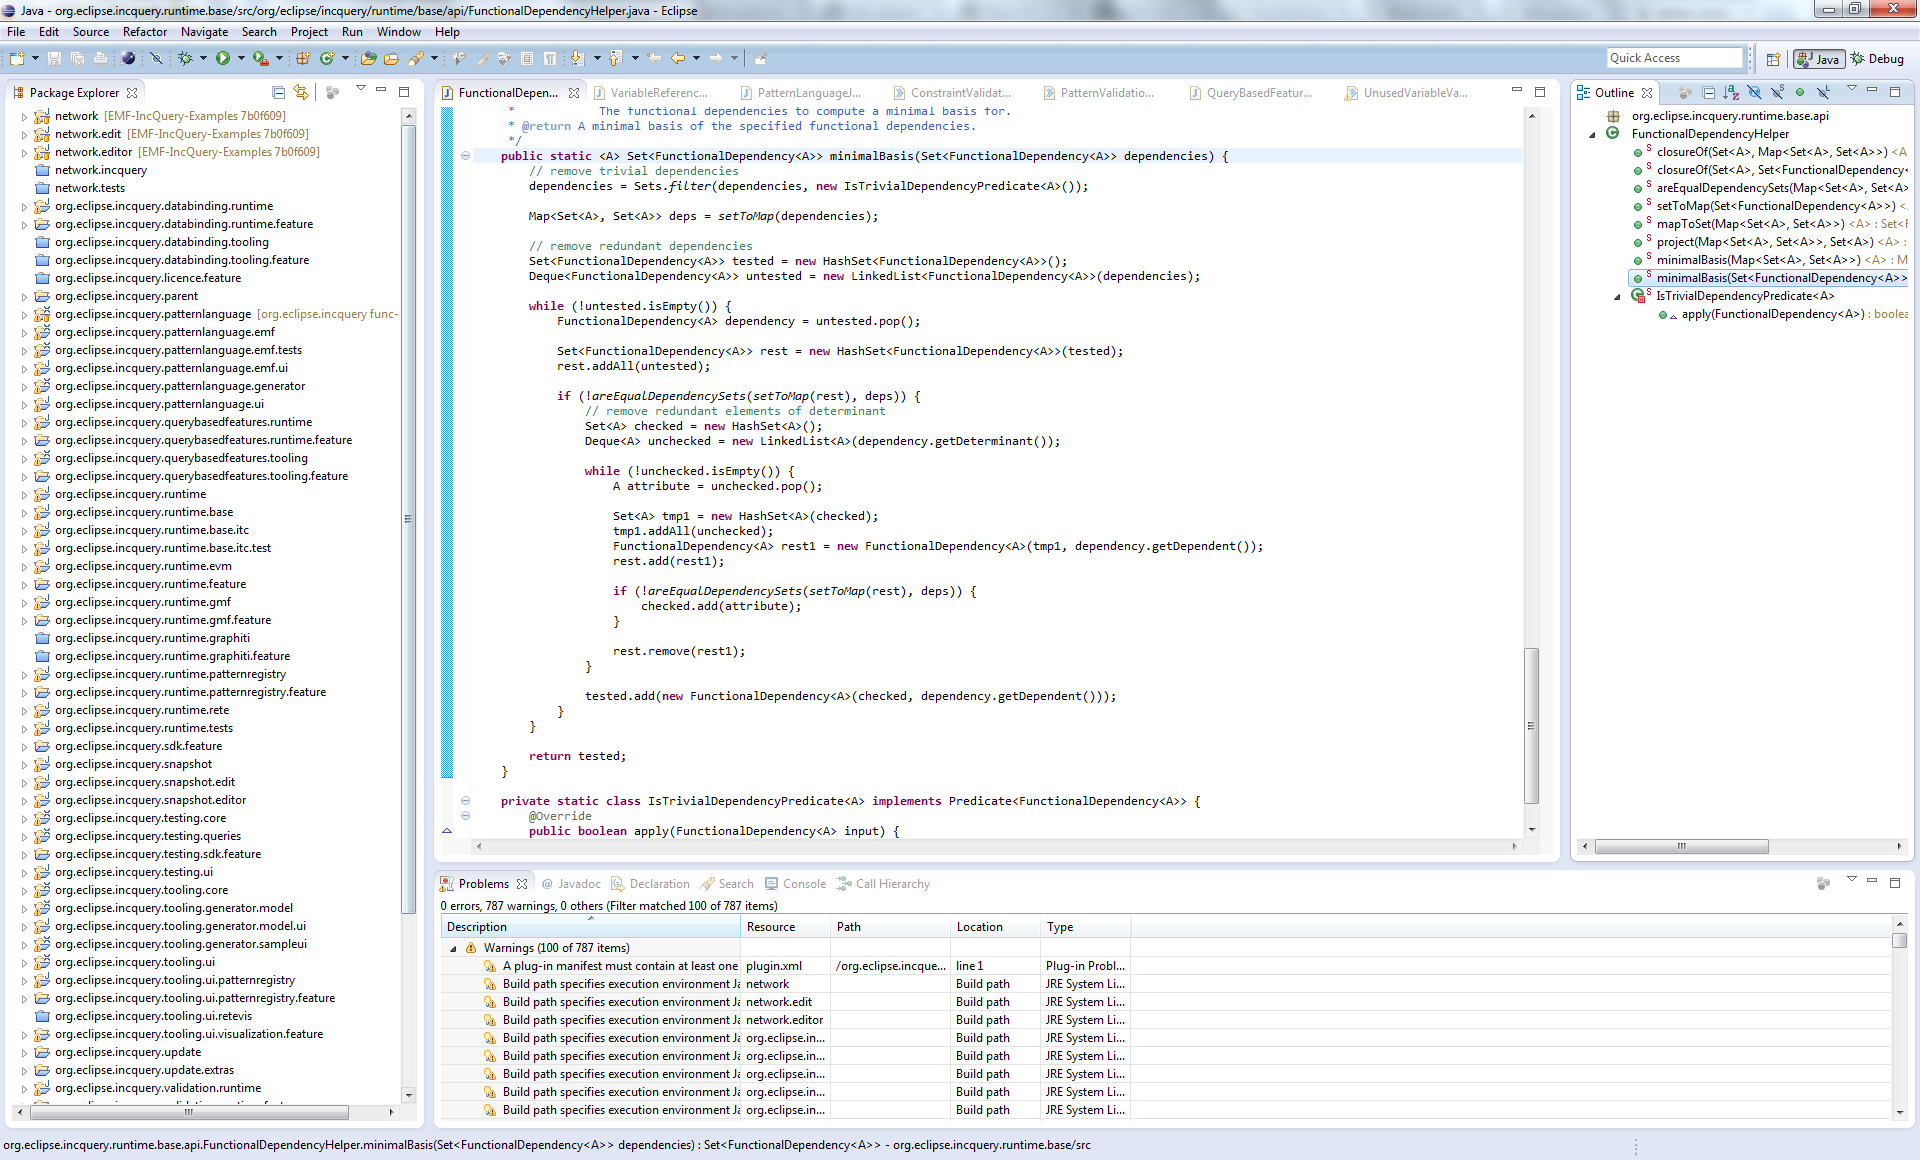
\includegraphics[width=\textwidth]{figures/eclipse-ide.png}
\caption{Eclipse fejlesztőkörnyezet Windows 7 operációs rendszeren}
\label{fig:EclipseIDE}
\end{figure}
%
Ilyen nyelvek többek között az Ada, C/\CPP, Clojure, COBOL, Erlang, FORTRAN, Haskell, JavaScript, Perl, PHP, Python, R, Ruby, Scala, Scheme.
Az Eclipse céljaiban hasonlít a Microsoft Visual Studio, vagy az Embarcadero Rapid Application Development (RAD) Studio integrált többnyelvű szoftverfejlesztő környezetére.
Platformfüggetlenségét Linux, Mac OS X, Solaris és Windows operációs rendszereken való futtathatósága jelenti.
A nyílt forráskódú környezet és hozzá kapcsolódó egyéb projektek rendszeres továbbfejlesztésről és új összetevők hozzáadásáról a lelkes és nyílt fejlesztői közösség  gondoskodik az Eclipse Foundation irányítása mellett.
%A legutóbbi 4.3 verzió a Kepler nevet viseli és 2013. június 26-án jelent meg, de már folyik a legújabb, Luna projekt is \cite{wiki:EclipseIDE}. 

Az integrált szoftverelemek felölelik a szoftverfejlesztés majd minden fázisát.
A fejlesztést szolgáló projektekről az Eclipse-közösség főoldaláról elérhető Projects (\url{http://projects.eclipse.org/}) lapon tájékozódhatunk.
A különböző fejlesztési fázisában lévő 235 fő- és alprojekt mutatja a kezdeményezés nagyságát.
A fő projektek között megtaláljuk a
\begin{itemize}
    \item Business Intelligence and Reporting Tools (BIRT)
    \item Data Tools Platform
    \item Eclipse Project
    \item Eclipse Modeling Project
    \item Mylyn
    \item RT
    \item SOA Platform Project
    \item Technology Project 
    \item Tools Project
    \item Eclipse Web Tools Platform Project
\end{itemize}
főágakat, melyek közül számunkra a dolgozat témája miatt legfontosabb az Eclipse Modeling Project főág a benne található Eclipse Modeling Framework (\gls{EMF}), \mbox{Xtext} és \mbox{VIATRA2} alprojektek miatt, mivel ezek kapcsolódnak legszorosabban az EMF-IncQuery-hez, de az Eclipse Project főág is említésre méltó.

Az Eclipse Project célja egy nyílt forráskódú, robusztus, általános célú, ipari színvonalú platform kidolgozása, mely magas szinten integrált komponensekkel segíti az alkalmazások fejlesztését.
Ennek eléréséhez nyújt támogatást a Plug-in Development Environment (PDE) Eclipse beépülő modulok és egyéb Eclipse platformra épülő eszközök kifejlesztésének elősegítésével.
Az alprojekt széleskörű \gls{OSGi} eszközkészletet is szolgáltat, mely ideális környezetté teszi komponens programozáshoz is a beépülő-modul fejlesztésen túl \cite{EclipseOrgPDE}.

Az EMF-IncQuery keretrendszernek részei olyan komponensek, melyek a PDE-et felhasználva beépülnek az Eclipse fejlesztői környezetbe, ahol varázslókkal és fejlesztési idejű ellenőrzésekkel támogatják lekérdezések definiálását az EMF-IncQuery szöveges tárgynyelvén vagy akár grafikus formában \cite{Gyorok13}, továbbá lehetővé teszik az elkészült lekérdezések interaktív futtatását \gls{EMF} példánymodelleken.

%----------------------------------------------------------------------------

\section{Az Eclipse Modeling Framework}

Az Eclipse Modeling Framework (\gls{EMF}) adatszerkezetek, domének modellezésére szolgáló keretrendszer, mely modell-vezérelt szoftverfejlesztést tesz lehetővé, vagyis képes a modellezett adatszerkezetek Java kódjának generálására is \cite{VogelEMF}.
Ily módon könnyen áttekinthető vizuális támogatással és grafikus szerkesztővel hozhatunk létre robusztus, nagyméretű adatrendszer modelleket, melyekből a közvetlen kódgenerálás is megoldott.
Az \gls{EMF} előnyei között említendő a csoportmunka támogatása is.
Az adatszerkezetek modellezésére vonatkozó ajánlás azok elkülönítése a programkódtól, ily módon csak adattagokat tartalmazó osztályok definiálása.

Az \gls{EMF} megkülönbözteti az adatmodell modelljét, azaz az adatmodell szerkezetét leíró meta-modellt az aktuális modelltől, mely a meta-modell egy példányaként fogható fel. 
Az \gls{EMF} modellező széles elterjedtségét magyarázza a magas szintű modellezés kivitelezésének könnyű volta, az erős integráltsága az Eclipse alá, továbbá az automatikus kódgenerálás.
Számtalan alkalmazása közül megemlítendő több Eclipse projektben való felhasználása.

A továbbiakban mélyebben elemzem az EMF szerkezetét és lehetőségeit az \url{http://www.eclipse.org/modeling/emf/docs/} weboldalon található áttekintő cikkek \cite{Steinberg:2009:EEM:1197540,VogelEMF} feldolgozása révén.

Meta-modellből kettő található az EMF-ben:
\begin{itemize}
	\item Ecore meta-modell és 
	\item Genmodel meta-modell.
\end{itemize}
Az Ecore meta-modell a definiált osztályokról tartalmaz információt, míg a Genmodel a Java kód generálásához tartalmaz járulékos adatokat, mint pl. fájlnevet és elérési utat, valamint a kódgenerálást vezérlő paramétert.
Az Ecore meta-modell különféle elemek definiálását teszi lehetővé:
\begin{itemize}
	\item \texttt{EClass}: attribútumokat és/vagy hivatkozásokat tartalmazó osztály
	\item \texttt{EAttribute}: névvel és típussal rendelkező attribútum
	\item \texttt{EReference}: két osztály közötti kapcsolat egyik végét reprezentálja; egy flag-gel jelzi, ha tartalmazást reprezentál
	\item \texttt{EDataType}: adattípus, pl. \texttt{int}, \texttt{float}, \texttt{java.util.Date}.
\end{itemize}
%
Az Ecore meta-modell felépítését a \ref{fig:EcoreStruct}. ábra mutatja.
%
\begin{figure}[htb]
\centering
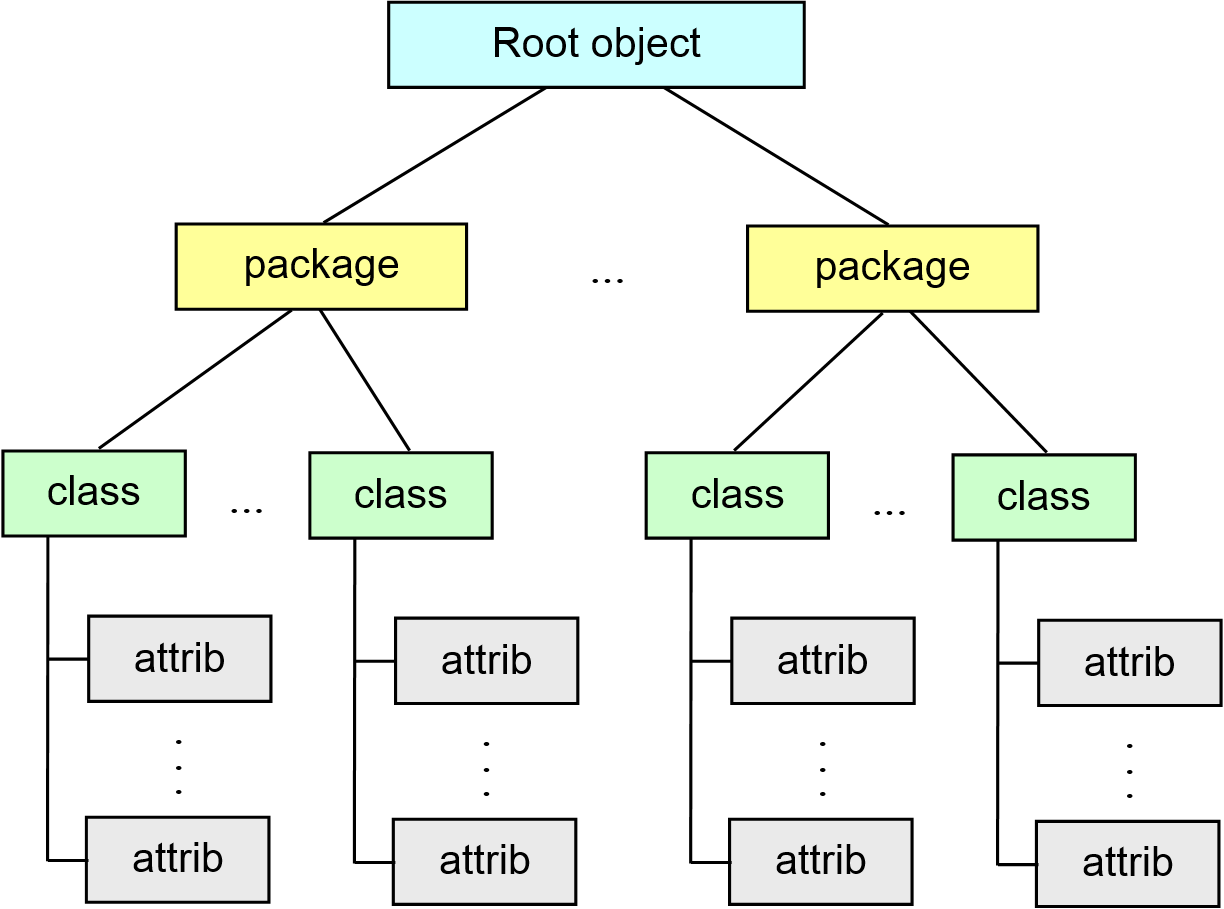
\includegraphics[width=0.8\textwidth]{figures/ecore-metamodel-struct.png}
\caption{Ecore meta-modell szerkezete}
\label{fig:EcoreStruct}
\end{figure}
%
Az Ecore meta-modell fő elemei a \ref{fig:EcoreStruct}. ábra kontextusába helyezve a következők \cite{EMFFundamentals}: 
A gyökér objektum egy EObject elem, ebbe tartoznak az EPackage csomagok, melyek egyszerre kezelendő osztályokból (EClass és EDataType) épülnek fel.
A class szinten EClass elemek reprezentálják a modellezett osztályokat, melyek a nevükből és EAttribute és/vagy EReference elemekből állnak.
Az attribútumoknak neve és típusa is van, míg a referenciák egy bináris kapcsolat egyik irányát modellezik, van nevük és megadják a hivatkozott osztály típusát és a tartalmazásjelző flag-et.
Az adattípust az EDataType elem adhatja meg.  

Az alkalmazások konkrét adatmodelljei az Ecore meta-modell egyedei.
A \ref{fig:DataModelWithXMI}. ábra mutat egy konkrét példát egy alkalmazás adatmodelljére.
%
\begin{figure}[htb]
\centering
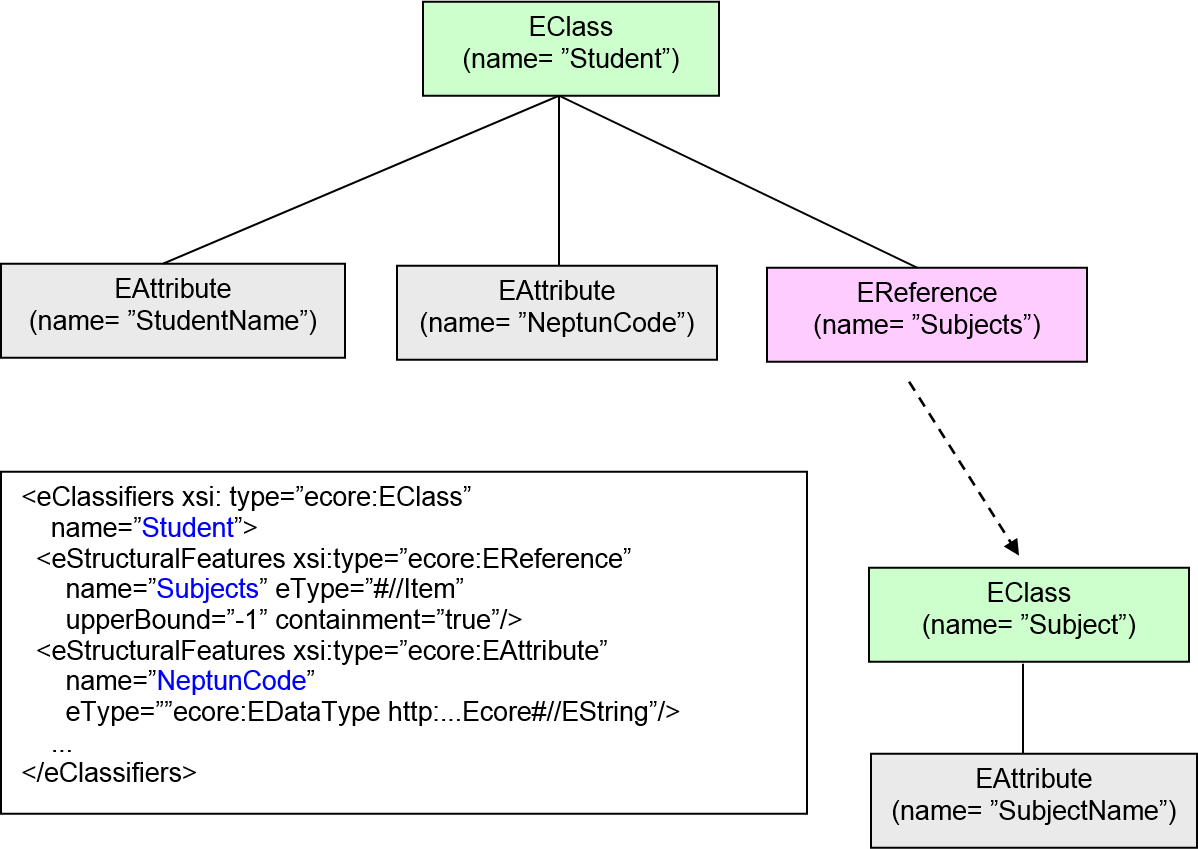
\includegraphics[width=\textwidth]{figures/datamodel-example-with-xmi-desc.png}
\caption{Alkalmazás adatmodell példa, XMI formátumú megadással}
\label{fig:DataModelWithXMI}
\end{figure}
%
Az EMF modell lényegében az UML osztálydiagram nézetének egy részhalmaza \cite{EMFFundamentals}.
Az EMF modellek az alábbi módokon is megadhatók:
\begin{enumerate}
	\item Java Interfaces
	\item UML Class Diagram
	\item XML Schema
\end{enumerate}
A modellimport és a kódgenerálás lehetőségeit a \ref{fig:ModelImportAndCodegen}. ábrán láthatjuk \cite{EMFFundamentals}.
%
\begin{figure}[!b]
\centering
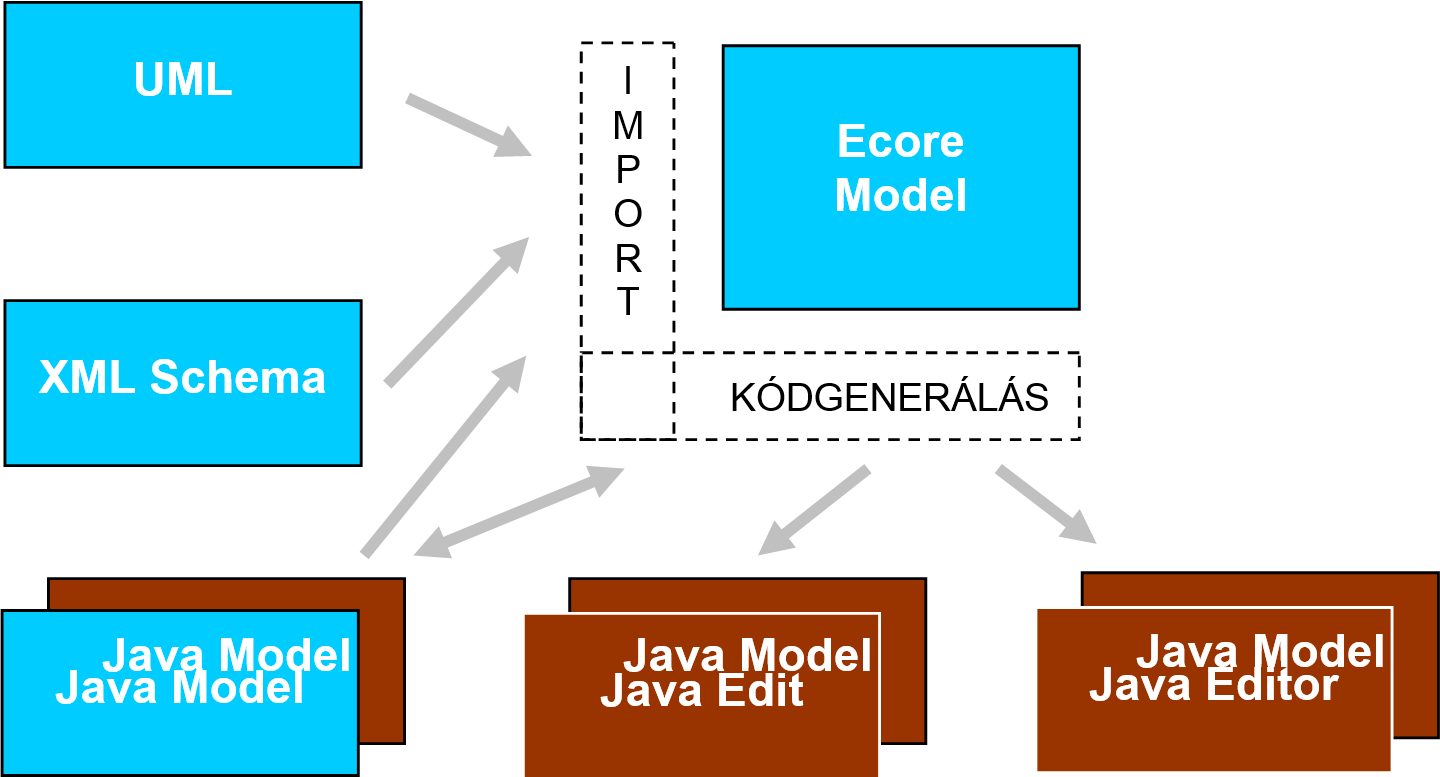
\includegraphics[width=\textwidth]{figures/model-import-and-codegen.png}
\caption{Modell import és kódgenerálás}
\label{fig:ModelImportAndCodegen}
\end{figure}
%
A kódgenerálás oda-vissza működik, Ecore modell generálható annotált Java interfészekből \cite{MasteringEMF}.
A generált kód tartalmazza az interfészt és az osztály implementációt, pl. a \ref{fig:DataModelWithXMI}. ábra szerinti modell esetén a következő formában:
%
\begin{lstlisting}
public interface Student extends EObject
{
    String getStudentName();
    void setStudentName(String value);
    String getNeptunCode();
    void setNeptunCode(String value);
    EList<Subject> getSubjects();
}
\end{lstlisting}
\begin{lstlisting}
public class StudentImpl extends EObjectImpl
    implements Student
{
    ...
}
\end{lstlisting}
A programkód tartalmazza a getter/setter elérőfüggvényeket az attribútumokhoz és a referenciákhoz.

Az EMF meta-modell létrehozását az \ref{fig:EcoreDiagramEditor}. ábra szerinti grafikus szerkesztő segíti.
%
\begin{figure}[htb]
\centering
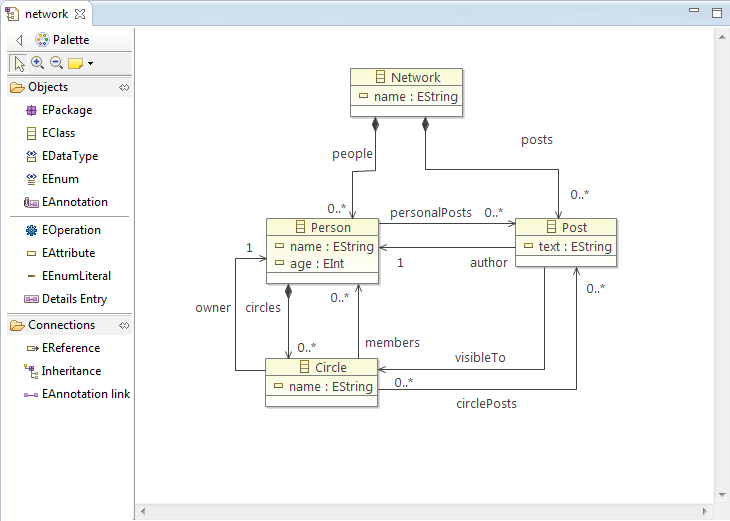
\includegraphics[width=\textwidth]{figures/ecore-diag-editor.png}
\caption{Ecore grafikus modellszerkesztő}
\label{fig:EcoreDiagramEditor}
\end{figure}
%
Egy példát egy adatszerkezetre \cite{VogelEMF} alapján a \ref{fig:EcoreMetaModelExample}. ábra mutat.
%
\begin{figure}[htb]
\centering
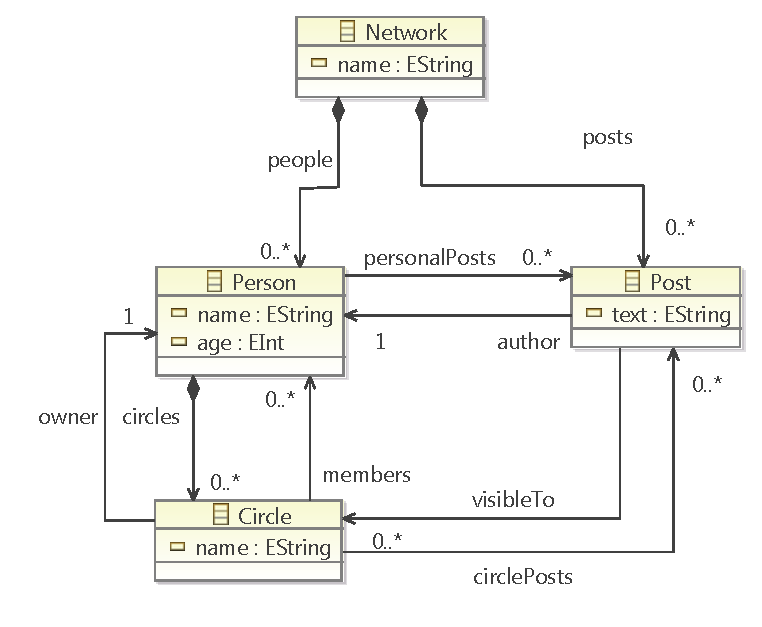
\includegraphics[width=\textwidth]{figures/ecore-network-metamodel-diag.pdf}
\caption{Példa Ecore meta-modellre (Network modell)}
\label{fig:EcoreMetaModelExample}
\end{figure}

A dolgozatban kulcsszerepet játszó Eclipse Modeling Framework (\gls{EMF}) bemutatásának összefoglalásaként a következőket emelhetjük ki \cite{EMFFundamentals}:
Az \gls{EMF} a legkézenfekvőbb modellező eszköz a Java környezet számára.
Az alkalmazás belső modelljére épít, nem szükséges más magas szintű modellező eszköz.
A modellezést és a programozást keverten is képes kezelni növelve ezáltal mindkettő hatásfokát.
A szoftverfejlesztés termelékenységét növeli és megkönnyíti az integrációt.
Mindezek alapján az Eclipse modell alapú fejlesztésének és adatintegrációjának az alapja. 

A feladatkiírás szerint az \gls{EMF}-re épülő, a Budapesti Műszaki Egyetem Méréstechnika és Információs Rendszerek Tanszékének Hibatűrő Rendszerek Kutatócsoportja által kidolgozott, modell-lekérdezések végrehajtására alkalmas EMF-IncQuery keretrendszerben kell vizsgálatokat végeznem, ezért a következőkben ezt a keretrendszert ismertetem.

%----------------------------------------------------------------------------

\section{EMF-IncQuery}\label{sect:IncQuery}

A szekció célja bemutatni az EMF-IncQuery és a lekérdezőnyelv felépítését, használatát, továbbá, a feladatkiírás első pontjának megfelelően, a modell-lekérdezések fogalmát az EMF-IncQuery keretrendszeren keresztül.

A keretrendszer főbb tulajdonságait röviden a \cite{EMFIncQuery} foglalja össze:
Az EMF-IncQuery \gls{EMF} modelleken végzendő deklaratív lekérdezések definiálására és végrehajtására alkalmas keretrendszer.
Fontos jellemzője, hogy a definiált lekérdezéseket kézi programírás nélkül, hatékonyan hajthatjuk végre.
A lekérdezőnyelv a gráfmintázatok módszerét alkalmazza, amely tömör és egyszerű eljárás komplex szerkezetű modell-lekérdezések megadására.
A kiemelkedő futási teljesítményt azáltal nyújtja, hogy inkrementális gráfminta illesztési technikákat alkalmaz.
Ennek köszönhetően a keresés még milliós nagyságrendű elemszám mellett is gyors.
Emellett az \gls{EMF} pár hiányosságát is orvosolja, mint például az osztályok egyedinek gyors és hatékony felsorolása helyre való tekintet nélkül, egyszerű fordított navigáció bármilyen referencia mentén, és objektumok megkeresése attribútum érték alapján.
Az újabb verzió képes származtatott tulajdonságok -- virtuális attribútumok és referenciák -- kiértékelésére is.

\subsection{Felépítés}

Az EMF-IncQuery felépítését a \ref{fig:EMFIncQueryStructure}. ábra mutatja \cite{Bergmann-TOOLS-2012}.
%
\begin{figure}[htb]
\centering
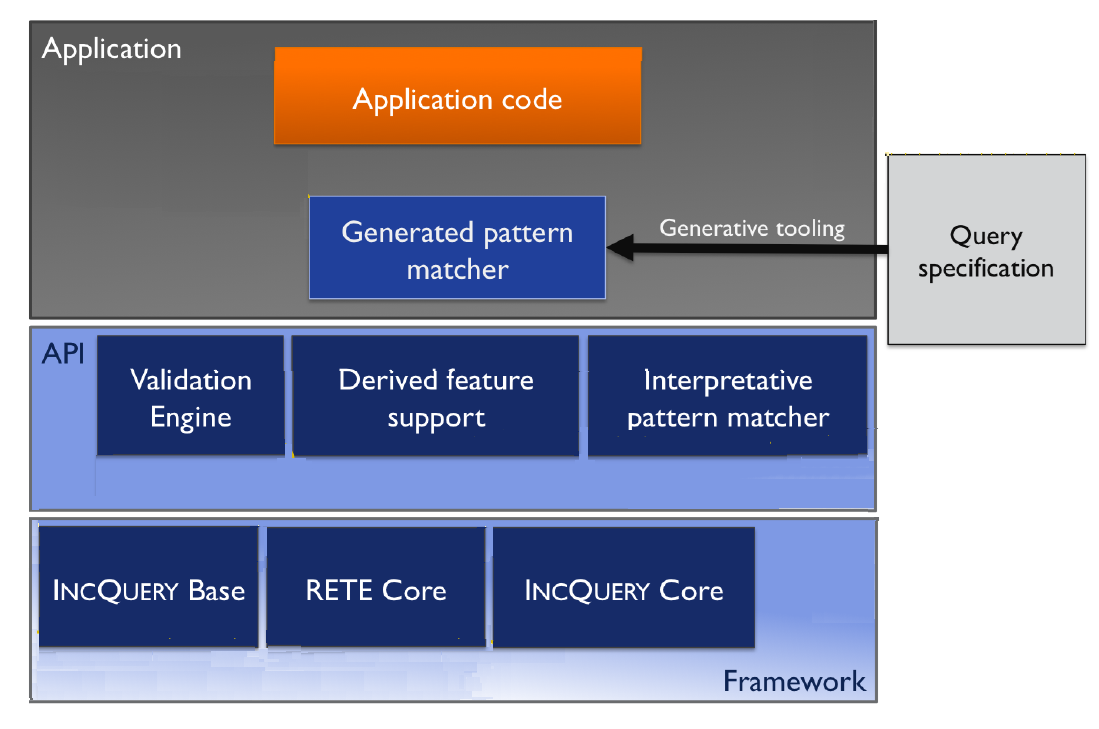
\includegraphics[width=\textwidth]{figures/emf-incquery-structure.png}
\caption{Az EMF-IncQuery felépítése}
\label{fig:EMFIncQueryStructure}
\end{figure}
%
A megadott lekérdezésen (Query specification) alapulva mintaellenőrző pluginok generálódnak (Generated pattern matcher), melyek könnyen integrálhatók egy meglévő Eclipse-alapú alkalmazásba (Application, Application code).
A lekérdezés megadását Xtext 2-alapú szerkesztő támogatja, amely fejlett szintaxis kiemeléssel, kódkiegészítéssel és formula ellenőrzéssel rendelkezik.
Ezek a pluginok az EMF-IncQuery API-n keresztül elérik a rendszer belső funkcionalitását.
Az API-ban a Validation Engine, validáló motor körbeveszi az EMF Validációs szolgáltatást  (Validation Service), hogy EMF-IncQuery-alapú online jól formáltság ellenőrzést végezve a validátorai révén szabványos Eclipse hiba markereket nyújtson.
Másodsorban az interpretáló mintaellenőrző (Interpretative pattern matcher) a Java kódból származó közvetlen lekérdezések számára elérési pontot nyújt azok gyors végrehajtásához.
Az API nyújtja továbbá a származtatott sajátosságok támogatását (Derived feature support).
A keretrendszerben a Base komponens gyakran használt alacsony szintű inkrementális lekérdezéseket nyújt, mint pl. a már említett egyed felsorolások, és fordított irányú navigálás egyirányú hivatkozásokon.
A lekérdezések inkrementális kiértékelését és életciklus kezelését a RETE motor szolgáltatja (RETE Core).
Az IncQuery Core adja az EMF-IncQuery keretrendszer magját.
A rendszer jellemzőinek mélyebb megértéséhez és az általa nyújtott szolgáltatások feltárásához a \cite{Bergmann-TOOLS-2012} irodalom volt segítségemre.

A gráfmintázatok keresése azzal az előnnyel jár, hogy a gráfminta által reprezentált feltételek vagy korlátozások a modellgráf megtalált, egyező mintázatú részén is teljesülnek.
A gráfminta strukturális, topológiai elvárásokat jelent, megadva az adott típusú élek és csomópontok kereséséhez az információt, továbbá kifejezésekkel az attribútumértékek iránt fogalmaz meg elvárásokat.
Egyes mintarészek/jellemzők kizárhatók az egyezés iránti elvárásból.
A gráfminta keresés ilyen módon nagyon finoman paraméterezett keresések kivitelezésére ad módot.

\subsection{Használat}

Ha egyszerűen csak használni szeretnénk az EMF-IncQuery által nyújtott szolgáltatásokat, akkor nem kell mást tennünk, mint telepíteni az \emph{EMF-IncQuery SDK}-t, illetve a hiányzó függőségeket a már meglévő Eclipse környezetünkbe \cite{EclipseOrgIncQueryInstall}.
Ha azonban újabb komponenseket szeretnénk a keretrendszerhez fejleszteni, akkor a \cite{EclipseOrgIncQueryDevEnv} forrás lesz a segítségünkre.
A fejlesztés megkezdéséhez először le kell tölteni a keretrendszer forráskódját, majd importálni a projekteket a fejlesztői környezetünkbe.
Ezután, az Xtext kódgeneráló munkafolyamatainak (MWE2 szkriptek) végrehajtásával előbb legeneráljuk a lekérdezőnyelv feldolgozásához szükséges kódot, majd javasolt a projekt tisztítása és teljes újrafordítása.
Az eredményt Eclipse Application-ként futtatva, egy olyan Eclipse fejlesztői környezet indul el, amelybe automatikusan betöltődnek az EMF-IncQuery moduljai.

Az így kapott környezetben kipróbálhatjuk az EMF-IncQuery-t: írhatunk lekérdezéseket a tárgynyelven, majd lefuttathatjuk őket példánymodelleken.
Ehhez azonban szükségünk lesz egy modellre.
Ha rendelkezünk már megfelelő EMF modellel, akkor használhatjuk azt, én azonban szeretném röviden bemutatni a modell elkészítésének menetét.

Mint modellezéskor mindig, most is egy domén specifikációjából fogunk kiindulni.
Az általam modellezett domén a karate harcművészetet űzők egy egyszerűsített világa lesz.
Ennek a világnak fő elemei a \emph{karatékák}, a karate harcművészek.
Minden karatékának van neve, és lehet egy meghatározott stílusa.
A karatékák lehetnek \emph{mesterek} vagy \emph{tanítványok}.
A tanítványok egy és csak egy mester alatt tanulhatnak, azonban a mestereknek nem szükségszerű, hogy legyen tanítványuk.
Minden mester a saját \emph{dódzsójában} (edzőterem, klub) oktatja tanítványait, melynek van neve.
Az előző két mondat állításaiból következik, hogy egy tanítvány egyszerre pontosan egy dódzsóban tanulhat.

Ezen leírás alapján elkészíthetjük a domén meta-modelljét az EMF Ecore diagram alapú modellezőjének segítségével.
Ennek mikéntjéről bővebb leírást a \cite{VogelEMF} ad.
Az általam elkészített meta-modellt a \ref{fig:karateMetaModel}. ábra mutatja.
%
\begin{figure}[htb]
\centering
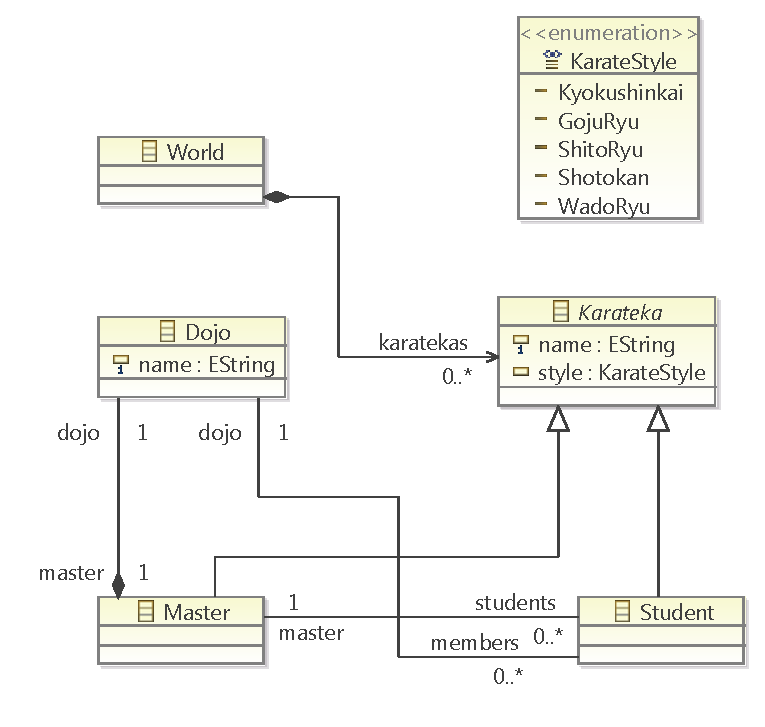
\includegraphics[width=\textwidth]{figures/ecore-karate-metamodel-diag.pdf}
\caption{Karate meta-modell}
\label{fig:karateMetaModel}
\end{figure}
%
Az ábrán látható diagram az UML osztálydiagramok jelölésrendszerét használja.
Jól láthatóak a kapcsolatok a modell főbb elemei közt: a Master és Student osztályok leszármazottjai az absztrakt Karateka osztálynak, megjelennek kétirányú kapcsolatok a Master, Student és Dojo osztályok között.
A KarateStyle a lehetséges karate stílusok felsorolása.
A modell gyökere a World osztály, ez tartalmazza a Karatekakat, akik közül a Master típusúak tartalmazzák a Dojokat.

Az Ecore meta-modell alapján elkészíthetjük a Genmodel meta-modellt, amelyből generálhatjuk modellünk egyedeinek létrehozásához és manipulálásához szükséges Java kódot és az Eclipse-be beépülő szerkesztő komponenseket, melyek segítenek a példánymodellek vizuális konstrukciójában.
A következő lépésben az elkészült komponenseket -- az EMF-IncQuery komponenseivel együtt -- betöltjük az Eclipse környezet egy újabb példányába a már említett módon (futtatás Eclipse Application-ként).
Itt varázsló segítségével létrehozhatjuk a modellünk egy új egyedét, melyet feltölthetünk a szükséges tartalommal.
Én a példánymodellemet a \emph{The Karate Kid} (A karate kölyök) című 1984-es kultuszfilm alapján készítettem el, töltöttem fel adatokkal.
Az elkészült példánymodellt fa formában a \ref{fig:karateInstanceModel}. ábra mutatja.
%
\begin{figure}[htb]
\centering
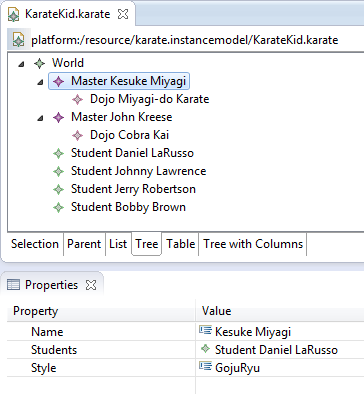
\includegraphics[width=0.70\textwidth]{figures/karate-instance-tree-with-properties.png}
\caption{Karate példánymodell}
\label{fig:karateInstanceModel}
\end{figure}
%

Példánymodellünk kész, jöhet a keresés!
A kereséshez szükségünk lesz egy gráfmintára.
Egy egyszerű, az EMF-IncQuery lekérdezőnyelvén megadott mintát láthatunk a \ref{lst:isStudentOfMiyagiPattern}. kódlistán.
%
\begin{lstlisting}[float,floatplacement=htb,caption=isStudentOfMiyagi gráfminta a tárgynyelven,label=lst:isStudentOfMiyagiPattern]
package karate.incquery

import "http://karate/1.0"

pattern isStudentOfMiyagi(student : Student) = {
    Student.master.name(student, "Kesuke Miyagi");
}
\end{lstlisting}
%
Ha a mintát beregisztráljuk az EMF-IncQuery \emph{Query Explorer} nézetébe és betöltjük mellé a példánymodellünket (\ref{fig:karateInstanceModel}. ábra) is, akkor a lekérdezés automatikusan kiértékelődik, és a \ref{fig:karateQueryResult}. ábrán látható eredményt kapjuk.
%
\begin{figure}[htb]
\centering

\includegraphics[width=\textwidth]{figures/karate-query-result.png}
\caption{Keresés eredménye}
\label{fig:karateQueryResult}
\end{figure}

\subsection{A lekérdezőnyelv}

A \ref{lst:isStudentOfMiyagiPattern}. kódlistán bemutatott keresési minta az EMF-IncQuery saját, deklaratív gráfminták leírására szolgáló nyelvén (IncQuery Graph Pattern language, IQPL) íródott, mely szintaxisának jelentős részét a VIATRA2 Textual Command Language-ből (VTCL) örökli, szemantikája pedig hasonló a Datalog deklaratív logikai lekérdezőnyelvéhez \cite{Ceri:1989:YAW:627272.627357}.

A nyelv feldolgozását a már említett Xtext keretrendszer végzi, mely programozási és doménspecifikus nyelvek fejlesztéséhez nyúlt alapot: az elemzéstől, a fordításon keresztül, a teljes Eclipse integrációig lefedi a szükséges nyelvi infrastruktúrát.
Az Xtext biztosít olyan eszközöket is, mint a szintaxis kiemelés, a kontextus alapú kiegészítés vagy a validáció.

A nyelv a következő fontosabb elemekből épül fel \cite{EclipseOrgIncQueryLang}:
\begin{description}
\item[Csomag:] a \texttt{package} direktíva -- a Java-hoz hasonlóan -- jelzi, hogy melyik csomag tartalmazza a fájlban lévő mintákat
\item[Importok:] \texttt{import} direktívákkal adhatjuk meg azokat az EMF csomagokat, melyeknek elemeire hivatkozni szeretnénk a lekérdezésekben
\item[Minta:] a \texttt{pattern} kulcsszóval bevezetett minták olyan \emph{predikátumok}, melyeknek lehetnek paramétereik -- melyeknek opcionálisan megadhatjuk a típusát is -- és legalább egy törzsük van; a minta törzsei diszjunktak, vagyis a törzsek logikai VAGY kapcsolatban állnak egymással
\item[Minta-törzs:] a kapcsos zárójelek által határolt minta-törzs legalább egy kényszerből és valahány lokális változóból áll; a törzsben lévő kényszerek logikai ÉS kapcsolatban állnak egymással 
\item[Kényszer:] kényszerek segítségével adhatóak meg a változók tulajdonságai és a közöttük lévő kapcsolatok; egy vagy több változóhivatkozás található bennük
\item[Változó:] értéke megadható, vagy mintaillesztésnél helyettesítődik be; a minta paramétereit \emph{szimbolikus}, a törzsekben találhatóakat pedig \emph{lokális} változóknak nevezzük
\end{description}

A kényszereknek az alábbi fajtái léteznek a nyelvben:
\begin{description}
\item[Összehasonlítás kényszer (\texttt{CompareConstraint}):] ez a kényszer két kifejezés egyenlőségét vagy egyenlőtlenségét határozza meg
\item[Típuskényszer (\texttt{EClassifierConstraint}):] ez a kényszer a paraméterének típusát határozza meg; példa: a \texttt{Student(student);} kifejezés a \texttt{student} változó típusát \textit{Student}-ként határozza meg
\end{description}
\todo{befejezni vagy törölni}
%----------------------------------------------------------------------------
\chapter{Változók használatának vizsgálata}
\label{chap:varUsage}
%----------------------------------------------------------------------------
%
% Bevezető
%
Az EMF-IncQuery lekérdezőnyelve -- más program- és leírónyelvekhez hasonlóan -- több olyan problémának is áldozatul esik, melyek statikus analízis segítségével hamar felismerhetőek, és a fejlesztők az analízis eredményét jó hatékonysággal használhatják fel az azonosított problémák orvoslására.
Az egyik leggyakoribb ilyen kellemetlenség a változók nevének (azonosítójának) nem konzisztens használata -- magyarul elírása -- a kód különböző pontjain, mellyel szinte minden informatikus találkozott már valamilyen formában.
A lekérdezőnyelv sajátossága miatt -- miszerint a lokális változókat nem szükséges előre deklarálni, mivel ezt a környezet impliciten, azok első előfordulásakor megteszi a fejlesztő helyett -- a kódban található kifejezések ilyen gépelési hibák elfordulása mellett is mindig szintaktikailag helyesek maradnak.
Így az ez által okozott hibák felderítéséhez a szemantikának, a kód jelentésének vizsgálatára van szükség, különben a hibára csak a lekérdezések futtatása után derülhet fény, melyre a rossz találati eredmények utalnak, és a hiba valódi oka még ekkor sem mindig egyértelmű.

%----------------------------------------------------------------------------
\section{Tervezés}

Az ilyen típusú ellenőrzés messze nem példa nélküli, más programozási nyelveknél és fejlesztőkörnyezeteknél gyakran találkozhatunk vele \emph{``nem használt változó detektálás''} néven.
Ám mivel az EMF-IncQuery lekérdezőnyelvében a változó fogalma kissé eltér a legtöbb nyelvben megszokottól, más környezetek megoldásai nem alkalmazhatóak egy az egyben.
Mint azt a \ref{chap:techPrim}. fejezetben már leírtam, a lekérdezőnyelv mintái esetében kétféle változóról beszélhetünk:
\begin{itemize}
    \item a \emph{paraméterváltozók}, melyek egy minta paraméterei, illetve
    \item a \emph{lokális változók}, amelyek egy mintának egy bizonyos törzsén belül fordulnak csak elő.
\end{itemize}
Ezek a változók leginkább az elsőrendű logika, illetve az ezen alapuló program- és lekérdezőnyelvek (pl. Prolog \cite{Colmerauer93thebirth}, Datalog \cite{Ceri:1989:YAW:627272.627357}) változóihoz hasonlíthatóak, így nem meglepő hogy beszélhetünk egy változó kvantifikáltságáról \cite{Huth:2004:LCS:975331}.

Mind a paraméterváltozók, mind a lokális változók lehetnek -- elméletben -- egzisztenciálisan vagy univerzálisan kvantifikálva, ám nem minden kombináció használható minden helyzetben, és a kétféle változókra valamelyest eltérő szabályok vonatkoznak.
A paraméterváltozóknak mindenképp felsorolható értékhalmazzal kell rendelkezniük, hiszen a mintaillesztőnek végső soron elő kell állítania az illeszkedések halmazát, ezen változókhoz is értéket rendelve.
Emiatt ezeknek a változóknak szükségszerűen egzisztenciálisan kvantifikáltaknak ($\exists x$) kell lenniük.
Univerzálisan kvantifikáltak ($\forall x$) nem lehetnek, hiszen akkor az összes elképzelhető modellentitásra kellene megvizsgálnunk a minta illeszkedését, ami pedig egy megoldhatatlan probléma, mivel ezek halmaza végtelen elemű, ugyanis az EMF-IncQuery szemantikája szerint az attribútumértékek is megköthetőek változóba.
Ugyanez a logika igaz általánosságban a lokális változókra is, egy kivétellel: a lokális változó lehet univerzálisan kvantifikálva, ha pontosan egy, \emph{negatívan alkalmazott} kényszerben szerepel.
A negatívan alkalmazott kényszerek negatív egzisztenciális kvantifikációt ($\neg\exists x$) jelentenek, ami az alábbi egyenlet alapján univerzális kvantifikációvá alakítható:
\begin{equation} \label{eq:negexiststoforall}
\neg\exists x\, P(x) \equiv \forall x\, \neg P(x)
\end{equation}
Ilyenkor a lokális változó ugyan univerzálisan van kvantifikálva, de az értékkészletét felsorolni sosem kell, hiszen egy negatív kényszerben szerepel, ami azt jelenti, hogy a kényszernek nem kell, sőt, nem is szabad teljesülnie.

Létezik még az úgynevezett \emph{read-only} kategóriába sorolható hivatkozás.
Ez olyan kifejezésekben fordul elő, ahol a kifejezés értéke alapján nem határozhatóak meg a kiértékelése során számba vett entitások.
Emiatt az ilyen kifejezéseket is univerzálisan kvantifikálónak tekinthetjük, mivel egzisztenciálisan nem kvantifikálják paramétereiket.
Ilyen kifejezések az ellenőrzés kényszerben lévő Java kifejezés és az aggregátor kifejezések.
%\todo{Az attribútumvizsgálat, pl. check (A<B) szerintem tök szemléletes további példa lenne itt, és jól elmagyarázható, hogy miért read only ez a változóhivatkozás}

A fent leírtakból következik, hogy \emph{egy paraméterváltozóra a minta minden törzsében lennie kell legalább egy egzisztenciálisan kvantifikáló hivatkozásnak}.
Egy lokális változó hivatkozásai két konstellációban fordulhatnak elő:
\begin{itemize}
    \item vagy egyetlen egy hivatkozás egy univerzálisan kvantifikáló, de negatívan alkalmazott kényszerben,
    \item vagy egy egzisztenciálisan kvantifikáló hivatkozás, illetve ezen kívül akárhány más hivatkozás
\end{itemize}
Az első esetben érdemes egyszer használatos változót alkalmaznunk, ami jelzi, hogy a változót máshol már nem szabad hivatkozni.
A második esetben szintén ajánlott egyszer használatos változót használnunk, \emph{ha} csak pontosan egy, egzisztenciálisan kvantifikáló hivatkozásunk van a változóra.
Ezzel jelezhetjük, hogy a változóra szándékosan nem hivatkozunk máshol.
Ellenkező esetben felmerülhet a kérdés, hogy a hivatkozás tényleg egy olyan új változót vezet be\footnote{Emlékeztető: a lokális változók első hivatkozásuknál impliciten deklarálódnak}, amelyre csak egyszer szerettünk volna hivatkozni, vagy a hivatkozás egy másik változóra irányult volna, de a változó nevét elgépeltük.

Tehát a változó típusától és a rá történő hivatkozások minőségétől és mennyiségétől függ, hogy a felhasználó milyen figyelmeztetést vagy hibaüzenetet kap, melyet részletesen az \ref{tab:warningsErrors}. táblázat mutat.
%
\tabulinesep=4pt
\begin{longtabu} to \textwidth{|X[1.5,c,m]|X[1,c,m]|X[1,c,m]|X[1,c,m]|X[3,c,m]|}
\caption{Figyelmeztetések és hibaüzenetek\label{tab:warningsErrors}} \\
\hline
& \multicolumn{3}{c|}{Változóhivatkozások a törzsben} & \\ \cline{2-4}
Változó & Pozitív & Negatív & Read-only & Üzenet típusa \\
\tabucline[1.5pt]{-}
\endfirsthead
\caption{Figyelmeztetések és hibaüzenetek (folyt.)} \\
\hline
& \multicolumn{3}{c|}{Változóhivatkozások a törzsben} & \\ \cline{2-4}
Változó & Pozitív & Negatív & Read-only & Üzenet típusa \\
\tabucline[1.5pt]{-}
\endhead
\multicolumn{5}{r}{\textit{a táblázat folytatódik a következő oldalon\ldots}} \\
\endfoot
\endlastfoot
Paraméter & 0    & 0    & 0    & Hiba: nincs hivatkozás a változóra \\
\hline
Lokális   & 1    & 0    & 0    & Figyelmeztetés: egyszer használt változó \\
\hline
Paraméter & 0    & 1    & 0    & Hiba: univerzálisan kvantifikált paraméterváltozó \\
\hline
Lokális   & 0    & 0    & 1    & Hiba: univerzálisan kvantifikált lokális változó \\
\hline
Paraméter & 0    & 0    & 1    & Hiba: univerzálisan kvantifikált paraméterváltozó \\
\hline
Lokális   & 0    & 0    & több & Hiba: univerzálisan kvantifikált lokális változó \\
\hline
Paraméter & 0    & 0    & több & Hiba: univerzálisan kvantifikált paraméterváltozó \\
\hline
Lokális   & 0    & 1    & 1    & Hiba: univerzálisan kvantifikált lokális változó \\
\hline
Paraméter & 0    & 1    & 1    & Hiba: univerzálisan kvantifikált paraméterváltozó \\
\hline
Lokális   & 0    & 1    & több & Hiba: univerzálisan kvantifikált lokális változó \\
\hline
Paraméter & 0    & 1    & több & Hiba: univerzálisan kvantifikált paraméterváltozó \\
\hline
Lokális   & 0    & több & 0    & Hiba: univerzálisan kvantifikált lokális változó \\
\hline
Paraméter & 0    & több & 0    & Hiba: univerzálisan kvantifikált paraméterváltozó \\
\hline
Lokális   & 0    & több & 1    & Hiba: univerzálisan kvantifikált lokális változó \\
\hline
Paraméter & 0    & több & 1    & Hiba: univerzálisan kvantifikált paraméterváltozó \\
\hline
Lokális   & 0    & több & több & Hiba: univerzálisan kvantifikált lokális változó \\
\hline
Paraméter & 0    & több & több & Hiba: univerzálisan kvantifikált paraméterváltozó \\
\hline
\end{longtabu}

%----------------------------------------------------------------------------

\section{Ellenőrzések}

Most lássunk néhány gyakorlati példát az eddig leírtakra.

\subsection{Hivatkozás nélküli paraméterváltozó}

Előfordulhat, hogy egy paraméterváltozóra nincs hivatkozás a minta egyik törzsében.

\begin{lstlisting}
package karate.incquery

import "http://karate/1.0"

pattern exampleQuery(student) = e_{
    Student(other);
    Student.name(other, "Daniel LaRusso");
}_
\end{lstlisting}
%
Ez hiba, mivel a változó így univerzálisan kvantifikálódik, ezért a mintaillesztő az adott törzs kiértékelésekor nem tud értéket rendelni a paraméterhez.

\subsection{Pozitív hivatkozás nélküli paraméterváltozó}

Előfordulhat az is, hogy van ugyan hivatkozás a paraméterváltozóra, de azok egyike sem (pozitív) egzisztenciális kvantifikáció.

\begin{lstlisting}
package karate.incquery

import "http://karate/1.0"

pattern notDaniel(student) = e_{
    neg Student.name(student, "Daniel LaRusso");
}_
\end{lstlisting}
%
% Megtévesztő, mert azt hinnénk hogy helyes, pedig nem.
%
vagy
%
\begin{lstlisting}
package karate.incquery

import "http://karate/1.0"
import "http://www.eclipse.org/emf/2002/Ecore"

pattern allStudents(student) = {
    Student(student);
}

pattern exampleQuery(student) = e_{
    EInt(n);
    n == count find allStudents(student);
}_
\end{lstlisting}
%
% Itt \texttt{s} csak bemeneti irányú (read-only) változó.
%
A probléma megegyezik az előző ellenőrzésnél látottal: a változó univerzálisan kvantifikált, a mintaillesztő nem tudja a változó értékhalmazát meghatározni.

\subsection{Lokális változó egyszeri hivatkozással}

Ha egy lokális -- de nem egyszer használatos -- változó csak egyszer kerül megemlítésre a kódban, akkor változók közti kapcsolat leírására nem szolgálhat -- ugyanis ahhoz legalább kétszer kellene szerepelnie.
Az ilyen helyzet elgépelésre vagy más hiányosságra utal.

\begin{lstlisting}
package karate.incquery

import "http://karate/1.0"

pattern isStudentOfMiyagi(student) = {
    Student(student);
    Student.master.name(w_studnet_, "Kesuke Miyagi");
}
\end{lstlisting}
,
\begin{lstlisting}
package karate.incquery

import "http://karate/1.0"

pattern studentsWhoHaveMaster(student) = {
    Student(student);
    Master(w_master_);
    // ez a sor maradhatott le: Student.master(student, master);
}
\end{lstlisting}
, illetve
%
\begin{lstlisting}
package karate.incquery

import "http://karate/1.0"

pattern allStudents(student) = {
    Student(student);
}

pattern numberOfStudents(n) = {
    EInt(n);
    n == count find allStudents(w_student_);
}
\end{lstlisting}

A fenti három esetben nem mondhatjuk egyértelműen, hogy hibázott a felhasználó, de szeretnénk felhívni a figyelmét a hibalehetőségre, ezért itt figyelmeztetést (warning) használunk.
Ha valóban csak helykitöltésre használjuk a változót -- mert nem érdekel minket például egy sok paraméteres minta néhány paramétere --, akkor használjunk anonim vagy egyszer használatos változót, hogy jelezzük szándékunkat és figyelmen kívül hagyjuk az ellenőrzést.

\subsection{Pozitív hivatkozás nélküli lokális változó}

Az egynél többször hivatkozott lokális változóknak, a paraméterváltozókhoz hasonlóan, szintén szükséges, hogy szerepeljenek legalább egy pozitív egzisztenciálisan kvantifikáló kifejezésben.
%
\begin{lstlisting}
package karate.incquery

import "http://karate/1.0"

pattern isShortName(name) = {
    Karateka.name(_, name);
    check(name.length < 10);
}

pattern longNamesExistThatAreNotMiyagi() = {
    neg find isShortName(e_name_);
    name != "Kesuke Miyagi";
}
\end{lstlisting}
%
Pozitív egzisztenciális kvantifikáció híján univerzálisan kvantifikálódik a \texttt{student} változó, így a mintaillesztő nem képes meghatározni értékhalmazát.

%----------------------------------------------------------------------------

\section{Implementáció}

A megtervezett ellenőrzés megvalósítását Java alapú Xtext validátor segítségével oldottam meg.
A validátor függvény egyetlen paramétere egy minta törzsét reprezentáló objektum, amelyen az ellenőrzést végezni fogja.
Az Xtext keretrendszer ezt a függvényt a validációs folyamat részeként minden ellenőrzésre kerülő minta összes törzsére egyenként meghívja.
A függvény egy mintatörzsben először megkeresi és minőségi csoportonként leszámlálja a törzsben és a törzshöz tartozó minta fejében található változóhivatkozásokat, majd az így felépített adatbázist bejárva megvizsgálja az egyes változókat a rájuk érvényes szabályok szerint, és ha szükséges, figyelmeztetést vagy hibaüzenetet emittál.
Az implementáció nem tér ki a tetszőleges Java kódot tartalmazó ellenőrzés kényszer és \texttt{eval} aggregátor kifejezés vizsgálatára, mivel az túlmutat a dolgozat keretein.

Az ellenőrzést működés közben a \ref{fig:unusedLive}. ábra mutatja.
\begin{figure}[!t]
\centering
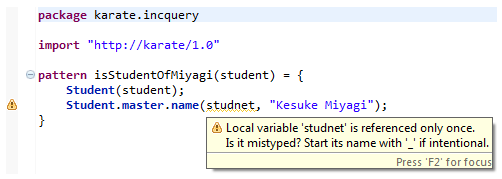
\includegraphics[width=0.90\textwidth]{figures/unused-variable-detection-warning.png}
\caption{Az elkészült ellenőrzés futás közben}
\label{fig:unusedLive}
\end{figure}

A validátor működésének teszteléséhez JUnit teszteket is készítettem, illetve frissítettem a már meglévő unitteszteket. Ezek segítenek a nyelv jövőbeni változása, bővítése miatt szükséges módosítások során az esetleges hibák megtalálásában (regresszió tesztelés), illetve valamilyen szinten bemutatják, biztosítják az elkészült ellenőrzések hatásosságát is.

%----------------------------------------------------------------------------
\chapter{Funkcionális függőség alapú vizsgálatok}
\label{chap:funcDep}
%----------------------------------------------------------------------------

Funkcionális függőségek vizsgálatával először a relációs adatmodell és a relációs adatbázisok tervezése kapcsán kezdtek el foglalkozni.
A relációs adatmodell a \emph{reláció} fogalmára épül -- mely (modell-)entitások valamilyen névvel ellátott kapcsolata --, és ezt egészíti ki a modellen elvégezhető műveletekkel.
Jó példa relációra a \ref{sect:IncQuery}. szekcióban leírt Karate doménünk \textbf{Master} és \textbf{Student} elemei között található \textbf{students} vagy \textbf{master} kapcsolat, de gyakoriak az olyan relációk is, melyek kettőnél több modell elem közötti kapcsolatot reprezentálnak.
Ennek szemléltetésére vegyük példaként egy karate verseny résztvevőit leíró relációt.
A reláció a következő attribútumokat tartalmazza:
\begin{itemize}
\item a versenyző neve (\textbf{Versenyző}),
\item a versenyző mesterének a neve (\textbf{Mester}), és
\item a versenyző dódzsója (\textbf{Dódzsó}).
\end{itemize}
Ennek a relációnak pár sorát láthatjuk a \ref{tab:karateTournamentCompetitorsRelation}. táblázatban.
%
\begin{table}[hbt]
\centering
\tabulinesep=6pt
\caption{Versenyzők adatai\label{tab:karateTournamentCompetitorsRelation}}
\begin{tabu} to \linewidth{|c|c|c|}
\hline
\rowfont{\bfseries}
Versenyző & Mester & Dódzsó \\
\tabucline[1.5pt]{-}
\everyrow{\hline}
\multicolumn{3}{|c|}{\ldots} \\
Bobby Brown & John Kreese & Cobra Kai \\
Daniel LaRusso & Kesuke Miyagi & Miyagi-do Karate \\
Johnny Lawrence & John Kreese & Cobra Kai \\
Jerry Robertson & John Kreese & Cobra Kai \\
\multicolumn{3}{|c|}{\ldots} \\
\end{tabu}
\end{table}
%
A táblázatot közelebbről megvizsgálva láthatjuk, hogy bizonyos mesterek és dódzsók több sorban is szerepelnek, méghozzá párban -- adott mester mellett mindig ugyanaz a dódzsó szerepel.
Ha feltesszük, hogy nincs két ugyanolyan nevű mester és tudjuk, hogy egy mester egyszerre csak egy dódzsóban tanít (a sajátjában), akkor azt mondhatjuk, hogy a \textbf{Mester} attribútum értéke egyértelműen meghatározza a \textbf{Dódzsó} attribútum értékét, vagyis minden olyan sorban, ahol megegyezik a \textbf{Mester} attribútumok értéke, a \textbf{Dódzsó} attribútumok értéke is meg fog egyezni.
Az ezt a jelenséget leíró matematikai konstrukciót nevezzük \emph{funkcionális függőségnek} (vagy függésnek)\cite{Gajdos06}.
Esetünkben azt mondhatjuk, hogy a \textbf{Dódzsó} attribútum funkcionálisan függ a \textbf{Mester} attribútumtól, vagy más szóval, a \textbf{Dódzsó} attribútum értéke származtatható a \textbf{Mester} attribútum értékéből, annak függvénye -- innen jön az elnevezés is.
Ahogyan a függvényeknek is lehet több bemeneti paramétere, úgy funkcionális függőségeknél is előfordul, hogy egy attribútumot több attribútum együttese határoz meg. (Gondoljunk csak arra, hogyan befolyásolja egy félév során történt számonkérések eredménye az év végi jegy alakulását egy tantárgyból.)
A későbbiekben ,,$X$ attribútum meghatározza $Y$ attribútumot'' kifejezésére az elterjedt $X \rightarrow Y$ jelölést használjuk, ahol a nyíl bal oldalán több attribútum is állhat, ha azok együttesen határozzák meg $Y$-t ($VWX \rightarrow Y$). Továbbá rövidítésként használjuk még a $WX \rightarrow YZ$ jelölést (több attribútum a nyíl jobb oldalán), mely alatt azt értjük, hogy a jobb oldalon álló attribútumok mindegyikét külön-külön is meghatározzák a bal oldalon álló attribútumok: $WX \rightarrow YZ \equiv WX \rightarrow Y \wedge WX \rightarrow Z$

Felmerül a kérdés, hogy ha rendelkezünk pár funkcionális függőséggel ($F$) egy reláció felett, akkor mi azoknak a függőségeknek a legbővebb halmaza, amely előállítható $F$ alapján.
Válaszként Armstrong 1974-ben publikálta azt a három axiómát (pontosabban következtetési szabályt), melyek segítségével generálhatjuk az összes olyan funkcionális függőséget, melyet $F$ implikál.
Az axiómák a következőek:
\begin{itemize}
    \item \textbf{reflexivitás}: ha $Y \subseteq X$, akkor $X \rightarrow Y$
    \item \textbf{tranzitivitás}: ha $X \rightarrow Y$ és $Y \rightarrow Z$, akkor $X \rightarrow Z$
    \item \textbf{bővíthetőség}: ha $X \rightarrow Y$, akkor $XZ \rightarrow YZ$
\end{itemize}
Az Armstrong axiómák és tulajdonságaik bővebb tárgyalása megtalálható a \cite{Gajdos06}-ben.

\emph{Triviális függőségnek} nevezzük azt az esetet, amikor egy attribútum önmagát határozza meg ($X \rightarrow X$).
Ez a függőség minden esetben teljesül Armstrong reflexivitás axiómája alapján.
Ehhez némileg hasonló az az eset, amikor egy attribútum egy konstans értéket határoz meg ($X \rightarrow k$, ahol $k$ egy konstans érték, például $42$ vagy \textit{,,alma''}).
Ez a függőség is bármikor teljesül, hiszen csak azt mondja ki, hogy $X$ bármely értéke mellett a konstans értéke önmaga marad, amely a konstans definíciójából természetesen következik.
Az ilyen függőségek esetén a konstansokat az üres halmazzal ($\varnothing$) szokás reprezentálni, hiszen nem tartalmaznak attribútumot: $X \rightarrow \varnothing$.
Ennek a fordítottja, mikor egy konstans érték határoz meg egy attribútumot ($k \rightarrow X$ vagy $\varnothing \rightarrow X$).
Ebben az esetben $X$ értéke is konstans lesz.

\section{Származtatott tulajdonságok}

Aki programozott már valamilyen objektum-orientált paradigmát támogató nyelven, annak minden bizonnyal ismerős az elérőfüggvények fogalma (\emph{getter} és \emph{setter}).
Aki ismer olyan nyelvet, amely támogatja, hogy ezeket a metódusokat a tulajdonság-eléréssel megegyező szintaxist használva érjük el, úgynevezett \emph{property}-ként -- ilyen nyelvek például: \CSharp, D, Delpi, Python --, az tudja milyen hasznos ez a funkcionalitás, melynek segítségével könnyedén illeszthetünk akár komolyabb logikákat egy egyszerű tulajdonság-elérés mellé, vagy ahelyett.
Az objektumok ezen tagjait szokás \emph{származtatott tulajdonságoknak} nevezni.

A származtatott tulajdonságok használatához az alábbi dolgokra van szükség:
\begin{itemize}
    \item az Ecore meta-modellen definiálni kell egy \texttt{EAttibute}-ot vagy \texttt{EReference}-t a kívánt névvel, típussal és multiplicitással, és beállítani a következő tulajdonságokat a létrejött \texttt{EStructuralFeature}-ön, hogy annak viselkedése megfelelő legyen: \textbf{derived} = \texttt{true}, \textbf{changeable} = \texttt{false}, \textbf{transient} = \texttt{true}, \textbf{volatile} = \texttt{true}
    \item definiálni kell a származtatás logikáját, és azt hozzárendelni a modellünkhöz
\end{itemize}
A tulajdonságok mögötti logikát a Genmodel meta-modellből generált Java forráskódhoz kell hozzáadnunk vagy kézzel, vagy valamilyen eszköz által generáltan.
Az egyik ilyen eszköz maga az EMF-IncQuery, melynek lekérdező nyelvében definiálhatunk egy mintát, amelyet a \texttt{QueryBasedFeature} annotációval megjelölve, a rendszer automatikusan generálja a szükséges kódot a minta alapján a megfelelő helyre. 
Ennek a technikának a részletes leírását a \cite{DerivedFeature} tartalmazza.
Az alábbi kódrészlet a \ref{sect:IncQuery}. szekció Karate modelljéhez definiál egy lekérdezést, amelynek segítségével automatikusan tudjuk biztosítani, hogy egy tanítvány dódzsója megegyezzen a mesterének dódzsójával.
%
\begin{lstlisting}
package karate.incquery

import "http://karate/1.0"

@QueryBasedFeature
pattern dojo(this : Student, result : Dojo) = {
    Student.master.dojo(this, result);
}
\end{lstlisting}
%
A minta neve (\texttt{dojo}) megegyezik a származtatni kívánt tulajdonság nevével.
A minta első paramétere (\texttt{this : Student}) a gazdaobjektum, melyen a származtatott tulajdonság található.
A minta második paraméterébe (\texttt{result : Dojo}) kerül majd maga a tulajdonság értéke -- ezért tekinthetünk rá úgy, mint egy kimeneti változóra, vagy egy függvény végeredményére.
A mintában lévő logika pedig a kapcsolatot írja le a gazdaobjektum és a tulajdonság között.

A fenti kódrészletben az annotáció alapértelmezett beállításait használjuk, ezért kötött a minta neve, és paramétereinek szerepe a pozíciójuktól függ.
Ezek a kötöttségek az annotáció megfelelő paraméterezésével természetesen feloldhatóak.
A \texttt{QueryBasedFeature} annotáció egyik paramétereként megadható a származtatott tulajdonság jellege (\emph{kind}), melynek értéke lehet egyes (\emph{single}), többes (\emph{many}), számláló (\emph{counter}), összeg (\emph{sum}) vagy iteráció (\emph{iteration}), és az alapértelmezett értéke a származtatott tulajdonság meta-modellben beállított multiplicitásának megfelelően egyes vagy többes.
A \texttt{QueryBasedFeature} annotáció paraméterezéséről bővebb tájékoztatást a \cite{DerivedFeature} ad.

Karate doménünkben kikötöttük, hogy egy tanítvány egyszerre csak egy dódzsóban tanul, tehát a tanítványok (\textbf{Student}) \textbf{dojo} tulajdonságának multiplicitása egyes.
A domén ezen tulajdonságát a meta-modell készítésekor is figyelembe vettem, ahogy az a \ref{fig:karateMetaModel}. ábrán is látható.
Ugyanezt a tulajdonságot tükrözi a fenti mintában található logika is, hiszen a meta-modell alapján minden tanítványnak pontosan egy mestere van, és minden mester pontosan egy dódzsóban tanít, tehát minden tanítvány pontosan egy dódzsóban kell hogy tanuljon.
A funkcionális függőség formalizmusát felhasználva a következőket mondhatjuk a tanítvány ($S$), mester ($M$), és dódzsó ($D$) attribútumok kapcsolatáról: a mester attribútum funkcionálisan függ a tanítvány attribútumtól ($S \rightarrow M$), a dódzsó attribútum funkcionálisan függ a mester attribútumtól ($M \rightarrow D$).
Ezekből Armstrong tranzitivitás-axiómáját felhasználva következik, hogy $S \rightarrow D$, vagyis a tanítvány attribútum funkcionálisan meghatározza a dódzsó attribútumot.
Ez, a funkcionális függőség definíciója szerint azt jelenti, hogy ugyanahhoz a tanítványhoz minden esetben ugyanaz a dódzsó fog tartozni, amit úgy is értelmezhetünk, hogy egy tanítvány pontosan egy dódzsóban tanulhat -- ahogyan azt a doménleírásunk alapján vártuk.

Láthatjuk, hogy a funkcionális függőség eszközével magából a logikából is meg tudjuk határozni egy származtatott tulajdonság multiplicitását.
Ez azonban -- a tárgynyelv felépítése miatt -- egy általánosan , ezért szükséges a multiplicitás manuális beállítása a meta-modellen.
Mi történik azonban akkor, ha rosszul álltjuk be ezt az értéket, vagy a logika módosítása után elfelejtjük azt frissíteni?
A legszerencsésebb esetben a modell többes jellegűként definiálja a tulajdonságot, azonban a származtatási logika miatt mindig csak legfeljebb egy érték kerül bele. Más esetekben az egyszerű csonkolástól a várt és kapott értékek típusának eltérése miatti futásidejű kivételig terjedő viselkedést kaphatunk.

\section{Származtatott tulajdonságok jellegének ellenőrzése}

Amint azt az előzőekben szemléltettem, hasznos információkhoz juthatunk az \gls{EMF} modellek és az EMF-IncQuery minták elemzésével a bennük található funkcionális függőségek szempontjából.
Az így kinyert információk segítségével figyelmeztethetjük a felhasználót ha ellentmondást találunk a modell és a logika között, illetve javaslatokat tehetünk a logika információtartalma alapján a modell javítására.
Én, az előző példában is bemutatott, származtatott tulajdonságok jellegének fejlesztési idejű ellenőrzését valósítottam meg egyes és többes jelleg esetén.
%\todo{mi a helyzet a többi jelleggel (counter, sum, iter)? -> főleg típus alapú ellenőrzések}

\subsection{Tervezés}

Az elkészült ellenőrzések mögötti logika megértéséhez előbb nézzük meg, mit is jelent egy származtatott tulajdonság egyes vagy többes jellege funkcionális függőségek szempontjából.
Ha a meta-modell egy eleme ($E$) és annak egy tulajdonsága ($A$) között funkcionális függés áll fenn ($E \rightarrow A$), akkor -- definíció szerint -- az elem egy adott egyedéhez mindig ugyanaz az érték fog társulni a tulajdonságban.
Vagyis az említett \emph{függőség fennállása esetén a tulajdonság jellege biztosan egyes}.
Ellenkező esetben, ha a függőség nem áll fenn -- vagy praktikusan nem dönthető el, hogy fennáll-e --, az azt jelzi, hogy a tulajdonság egyrészt esetenként különböző, másrészt akár több értéket is felvehet, ám ez nem garantált még akkor sem, ha a függőség bizonyítottan nem áll fenn.
Tehát ha valahogyan sikerülne szert tennünk az entitás és a tulajdonság közt fennálló funkcionális függőségekre, akkor az ezek alapján számított jelleget összevetjük az Ecore modellben definiált tulajdonságnál manuálisan megadott multiplicitással, és eltérés esetén figyelmeztethetjük a fejlesztőt.
A leírtakat a \ref{tab:funcDepVsModelMulti}. táblázat szemlélteti.
\begin{table}[hbt]
\centering
\renewcommand{\arraystretch}{1.5}
\caption{Funkcionális függőség és tulajdonság multiplicitás közti kapcsolat\label{tab:funcDepVsModelMulti}}
\begin{tabular}{|c|c|c|}
\hline
\diagbox{multiplicitás}{$E \rightarrow A$} & {\renewcommand{\arraystretch}{1}\begin{tabular}{c}nincs\\ (vagy nem\\ eldönthető)\end{tabular}} & van \\
\hline
1 & figyelmeztetés & \checkmark \\
\hline
* & \checkmark & figyelmeztetés \\
\hline
\end{tabular}
\end{table}

Mivel az entitás és a származtatott tulajdonság kapcsolatát esetünkben egy EMF-IncQuery minta, az abban található logika írja le, ezért a keresett funkcionális függőségek is ebben találhatóak.
A feladatunk tehát a \texttt{QueryBasedFeature} annotációval megjelölt minta paraméterei között fennálló funkcionális függőségek felderítése, melyhez szükségünk lesz a minta egyes törzseiben található funkcionális függőségek összegyűjtésére.
A minta egy adott törzse egy vagy több kényszerből áll, melyek logikai ÉS kapcsolatban állnak egymással, tehát ha a minta-törzs illeszkedik, akkor az összes benne lévő kényszer is teljesül.
Emiatt a törzsben fennálló funkcionális függőségek halmaza a törzsben található kényszerek által egyenként meghatározott funkcionális függőséghalmazok uniója.
Járjuk hát végig az előforduló kényszertípusokat, melyik milyen funkcionális függéseket rejt a paramétereire nézve.

Funkcionális függőségek szempontjából a legegyszerűbben elemezhető kényszer a \emph{típuskényszer} (\texttt{EClassifierConstraint}).
Ez a kényszer egyetlen paraméterének egyedül a típusát határozza meg, ami -- az egyke (singleton) típusokat kivéve -- nem határoz meg funkcionális függőséget.
Az egyke típusok felismeréséhez szükséges kardinalitás információt a rendszer sajnos nem szolgáltatja, így ezt nem tudtam kihasználni a függőségek összegyűjtésekor.

Második a sorban az \emph{összehasonlítás kényszer} (\texttt{CompareConstraint}), mely két kifejezés egyenlőségét vagy egyenlőtlenségét mondja ki.
Míg egyenlőség esetén a két kifejezés ($X$ és $Y$) kölcsönös függésben áll ($\left\{ X \rightarrow Y , Y \rightarrow X \right\}$), addig egyenlőtlenség esetén semmilyen függőséget nem tudunk meghatározni a kettő közt.
A két kifejezés bármelyike lehet érték\footnote{Pontosabban érték literál vagy kiértékelt hívás (pl. \texttt{count find \ldots}) értéke.} vagy változó, így három különböző kombináció állhat elő:
\begin{enumerate}
    \item két változó esetén: $\left\{ X \rightarrow Y, Y \rightarrow X \right\}$
    \item egy változó és egy érték esetén: $\left\{ X \rightarrow \varnothing, \varnothing \rightarrow X \right\}$
    \item két érték esetén: $\left\{ \varnothing \rightarrow \varnothing \right\}$
\end{enumerate}
A 2. kombinációból az $X \rightarrow \varnothing$ függőség elhagyható, hiszen az egyébként is mindig fennáll.
A 3. kombináció pedig teljesen elhagyható, mivel nincs információtartalma (triviális).

\begin{sloppypar}
Következő elemzett kényszertípusunk legyen az \emph{útvonal-kifejezés kényszer} (\texttt{PathExpressionConstraint}).
Ez a kényszer a meta-modell egy vagy több éle mentén állít fel kapcsolatot két paramétere közt.
A kényszer által meghatározott funkcionális függőség az egyes élek által meghatározott függőségek kompozíciójaként számítható.
Például \texttt{Student.master.dojo(E, A)} kényszer a \textbf{Student} és a \textbf{Master} típusú entitások között teremt kapcsolatot a \textbf{master} nevű élen, illetve a \textbf{Master} és a \textbf{Dojo} típusú entitások között a \textbf{dojo} nevű élen.
Egy segédváltozó (\texttt{T}) bevezetésével akár szét is bontható két egyszerűbb kényszerre: \texttt{Student.master(E, T)} és \texttt{Master.dojo(T, A)}.
Ez a lépés minden egynél több élet tartalmazó kényszer esetén megtehető.
Egy él mentén két függés állhat fent: egy az eredeti és egy másik a fordított irányban.
Az eredeti irányban akkor áll fenn funkcionális függés az entitás és a tulajdonság között, ha a tulajdonság multiplicitása egyes.
A fordított irányban egyrészt akkor állhat fenn függés, ha az eredeti él tartalmazást fejez ki, hiszen ekkor egyértelműen meghatározható az a pontosan egy entitás, ami tartalmazza a tulajdonság értékét.
Másrészt ha az él eleve kétirányú -- vagyis van ellentettje (eOpposite) a tulajdonságnak --, és az ellentett tulajdonság multiplicitása egyes.
Esetünkben a \textbf{master} és a \textbf{dojo} tulajdonságok multiplicitása is egyes, továbbá a \textbf{dojo} tulajdonság tartalmazást fejez ki.
Ezek alapján a következő függőségek írhatóak fel: $\left\{ E \rightarrow T, T \rightarrow A, A \rightarrow T \right\}$
Ebből Armstrong tranzitivitás axiómáját felhasználva és az eredményt a valódi változókra vetítve pedig következik, hogy $E \rightarrow A$.
Láthatjuk, hogy mivel a \textbf{master} tulajdonság ellentettje (\textbf{students}) többes multiplicitású, azon az élen a funkcionális függés nem áll fenn, így a tranzitivitási lánc megszakad a visszafelé irányban, így az a függőség ($A \rightarrow E$) nem teljesül.
\end{sloppypar}

A \emph{hívás} vagy más néven \emph{minta kompozíciós kényszer} (\texttt{PatternCompositionConstraint}) funkcionális függőségei a hívott minta által meghatározott funkcionális függőségekkel egyeznek meg akkor, ha a hívás nem negatív.
Negatív hívás esetén, az egyenlőtlenséghez hasonlóan, nem tudunk funkcionális függőségeket meghatározni.
Ebben az esetben tehát csak annyi a feladatunk, hogy a hívott minta funkcionális függőségeit rekurzívan meghatározzuk, majd a paraméterek pozíciója alapján leképezzük azokat a hívó minta változóira.

\begin{sloppypar}
Az utolsó kényszertípus, amiről még nem esett szó, az \emph{ellenőrzés kényszer} (\texttt{CheckConstraint}).
Ezzel a minta változóinak konkrét értékeire tehetünk megkötéseket -- akár tetszőleges komplexitású -- Java kifejezések segítségével.
Ezeknek a Java kifejezéseknek funkcionális függőségek szempontjából történő általános elemzése túlmutat a szakdolgozat keretein, így ezzel a problémával nem foglalkoztam.
\end{sloppypar}

Ezzel -- a dolgozat írásának pillanatában -- az összes lehetséges kényszertípust megvizsgáltuk a belőlük kikövetkeztethető funkcionális függőségek szempontjából.
Mint azt már írtam, a minta-törzs által meghatározott funkcionális függőséghalmaz egyszerűen a törzsben található kényszerek funkcionális függőségeinek összessége (uniója).
Egy minta állhat egy vagy több, egymással logikai VAGY kapcsolatban álló törzsből.
Egy törzs esetén a minta funkcionális függőséghalmazának meghatározásához a törzs függőséghalmazát vetíteni kell a minta paramétereire, hogy a kapott halmazban ne szerepeljenek a törzs lokális változói, melyek a törzs kontextusán kívül értelmezhetetlenek.

Több törzs esetén, a köztük fennálló logikai VAGY kapcsolat miatt, a funkcionális függőségek meglétén kívül szüksége van azok minőségére is, vagyis arra, hogy milyen élek mentén teljesül a függőség.
Egy rövid példával illusztrálom, miért van erre szükség.
Nézzük meg a funkcionális függőségeket a \ref{lst:multiBodyPattern}. kódlistán látható, családfa modellhez írt mintában!
\begin{lstlisting}[float,floatplacement=htb,caption=Példa több törzsű mintára,label=lst:multiBodyPattern]
package karate.incquery

import "http://karate/1.0"

pattern parentOf(child, parent) = {
    Person.mother(child, parent);
} or {
    Preson.father(child, parent);
}
\end{lstlisting}
A minta mindkét törzsében függ a \texttt{parent} változó értéke a \texttt{child} változó értékétől, hiszen minden embernek pontosan egy-egy -- biológiai -- anyja és apja van. Ugyanakkor egyszerűen belátható, hogy adott \texttt{child} paraméter mellett a \texttt{parent} változó két értéket is fel fog venni.
Az általam készített megoldás kibővítése ezeknek az eseteknek a kezelésével, egy remek önálló feladat lenne.

\subsection{Implementáció}

Az ellenőrzéseket Xtext validátor formájában implementáltam, pontosabban a már meglévő, \texttt{QueryBasedFeature} annotációk ellenőrzését végző validátor kódjába illesztettem be az általam készített részeket.
Az ellenőrzések elvégzéséhez egyrészt szükség volt a minták részeinek (minta, minta-törzs, kényszerek) elemzését elvégző segédfüggvényekre, melyek szinte triviálisan következnek az elméleti részben leírtakból.
Másrészt szükség volt a kinyert funkcionális függőségek reprezentálására és azokon különböző műveleteket elvégző függvények elkészítésére.
Az alábbi műveleteket valósítottam meg:
\begin{itemize}
    \item attribútumhalmaz lezártjának képzése adott funkcionális függőségek mellett
    \item függőséghalmazok ekvivalenciájának eldöntése
    \item funkcionális függés levezethetőségének (implikáció) eldöntése adott függőséghalmaz mellett
    \item függőséghalmaz vetítése adott attribútumhalmazra
    \item minimális függéshalmaz előállítása adott függéshalmazból
\end{itemize}

Mivel a funkcionális függőségek bármilyen típusú attribútumokat tartalmazhatnak, ezért a kapcsolódó adatstruktúrákat és metódusokat generikusan valósítottam meg, így azok nem csak a szakdolgozat részeként elkészült komponensben, hanem a keretrendszer más részeiben is felhasználhatóak lettek (például ahogyan azt a \ref{sect:caseStudy}. szekcióban részletezem).

Az elkészült ellenőrzés tesztelésére ideiglenesen módosítottam a Karate meta-modell (\ref{fig:karateMetaModel}. ábra) \textbf{Master} osztály \textbf{dojo} attribútumának multiplicitását 1-ről 1..2-re, vagyis megengedtem, hogy a mesterek esetleg egy második dódzsót is üzemeltessenek.
Ennek hatását az előzőekben bemutatott \texttt{dojo} lekérdezésre a \ref{fig:funcDepManyWarning}. ábra mutatja.
\begin{figure}[htb]
\centering
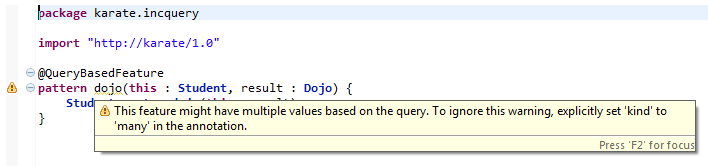
\includegraphics[width=\textwidth]{figures/func-dep-many-warning.png}
\caption{Multiplicitás eltérésre figyelmeztető üzenet}
\label{fig:funcDepManyWarning}
\end{figure}

%----------------------------------------------------------------------------

\section{Esettanulmány}
\label{sect:caseStudy}

Egy adott minta-törzsben található kényszereket (vagy egy részhalmazukat) kielégítő értékek $n$-esének keresését elképzelhetjük úgy, mintha egy $n$ oszlopú táblázat sorain vizsgálnánk egyesével, hogy az adott sorban lévő mezők értékeit behelyettesítve a kényszerek $n$ db változójába, azok teljesülnek-e.
Az ilyen táblázatokat, a relációs adatbázisok működéséhez hasonlóan, általában több kisebb táblázat egymáshoz \emph{illesztésével} (join) kapjuk.
A relációs adatbázisok fejlesztése során már rájöttek, hogy sok múlik ezeknek a műveleteknek a teljesítményén, ezért sok heurisztikát fejlesztettek ki az illesztések lehető leggyorsabb végrehajtásának biztosítására.
Az EMF-IncQuery keresőmotorja is alkalmaz ilyen heurisztikákat, melyek segítségével eldönti, hogy egyáltalán szükséges-e két tábla illesztése, illetve az illesztések mely sorrendje mellett lesz a teljesítmény optimális.

Az egyik ilyen heurisztika a funkcionális függőségeken, pontosabban a funkcionális függőség mentén történő \emph{veszteségmentes felbontás tételén} -- más néven Heath tétele -- alapszik.
A tétel kimondja, hogy ha egy $U$ attribútumhalmaz feletti relációra ($R(U)$) teljesül az $X \rightarrow Y$ függés (ahol $X$ és $Y$ attribútumhalmazok és $XY \subset U$), akkor a relációt e függés mentén felbonthatjuk két másik relációra ($R_1 = \pi_{XY}(R)$ és $R_2 = \pi_{XZ}(R)$, ahol $Z = U \setminus XY$, $\pi$ pedig a vetítés művelete) úgy, hogy a kapott relációk természetes illesztésével visszakapjuk az eredeti relációt ($R = R_1 \bowtie R_2$).
A heurisztika az előzőekben tárgyalt statikus, funkcionális függőség alapú vizsgálatokhoz készített, a függőségeket kezelő eszközöket hasznosítja.

Az EMF-IncQuery keretrendszer bemutatásához és teljesítményének méréséhez egyik gyakran használt domén-modell a \emph{Network} modell (\ref{fig:EcoreMetaModelExample}. ábra).
A modellhez három példánymodell készült: egy kicsi (1000 Person, 1000 Post és minden Person-höz 2 Circle), egy közepes (1000 Person, 1000 Post és minden Person-höz 10 Circle) és egy nagy (2000 Person, 2000 Post és minden Person-höz 20 Circle).

A modellhez írt lekérdezések egyike a \ref{lst:mutualFriendsPattern}. kódlistán látható.
\begin{lstlisting}[float,floatplacement=htb,caption=MutualFriends minta,label=lst:mutualFriendsPattern]
package network

import "http://network/1.0"

pattern MutualFriends(person: Person, friend: Person) = {
	person != friend;
	Person.circles.members(person, friend);
	Person.circles.members(friend, person);
}
\end{lstlisting}
Ennek a lekérdezésnek az egyik sajátossága, hogy naiv módszerrel történő kiértékelése rengeteg illesztési műveletet igényel, és eközben nagy táblákat hoz létre.

Az EMF-IncQuery Java virtuális gépen fut, így annak automatikus memóriakezelését használja -- a szemétgyűjtés módszerét (garbage collection).
A szemétgyűjtő működésének elve, hogy periodikusan vagy memóriahiány esetén megkísérli felszabadítani a memóriának azt a részét, amelyet az alkalmazás már nem használ.
Ha a program gyakran foglal le sok memóriát és azt csak rövid ideig használja, akkor a szemétgyűjtőnek gyakran kell lefutnia, hogy ki tudja elégíteni az alkalmazás újabb és újabb memóriaigényeit.
 
Méréseim során a közepes és a nagy példánymodelleken a fenti lekérdezés a Heath tételén alapuló heurisztika nélkül valamivel több, mint 4GB maximális memóriahasználat engedélyezésével sem futott le sikeresen egy-két órán belül.
A heurisztika engedélyezése után a közepes példánymodellen átlagosan 3 másodperc alatt futott le a lekérdezés, amihez 0,5GB memóriát használt fel. A nagy példánymodellen a lekérdezés átlagosan 16 másodperc alatt futott le és 1,5GB memóriát igényelt.
A mérések természetesen különböző hardvereken eltérőek lehetnek, ám az elért -- végtelenszeres -- teljesítmény növekedés egyértelmű.

%----------------------------------------------------------------------------
\chapter{Összefoglalás}
\label{chap:summary}
%----------------------------------------------------------------------------

A modell-vezérelt szoftverfejlesztés egy olyan széles körben elterjedt technológia, mely elősegíti az összetett szoftverrendszerek tervezését, készítését, továbbfejlesztését és karbantartását.
A technológia domének modellezésére és a modellek automatizált transzformációjára épít.

A szakdolgozat elkészítése során megismerkedtem a modellezés és modell-vezérelt szoftverfejlesztés technikáival, és az ezt támogató Eclipse integrált fejlesztői környezettel, és Eclipse Modeling Framework technológiával.

Megismertem a statikus analízis módszereit és lehetőségeit a szoftverfejlesztés hatékonyságának javítására.
  lekérdezések szöveges leírására szolgáló nyelvével és annak használatával, és az Xtext validátorok írásával.
Elemeztem a nyelvben statikus analízis segítségével megoldható problémák témakörét, és kiválasztottam ezek közül egy gyakran előforduló és kellemetlen következményekkel járó problémát, melynek kezelése mégis egyszerű, \sout{a féléves munka során megvalósítható}.
A probléma okának és körülményeinek mélyebb megismerése után megterveztem és megvalósítottam a megoldáshoz szükséges ellenőrzést.
Az elkészült alkotást működés közben a ~\ref{fig:unusedLive}. ábra mutatja.
\sout{Ugyan éles bevetésére még nem került sor}, az EMF-IncQuery fejlesztői és felhasználói már most élénk érdeklődést mutatnak iránta.

Az alábbi célokat értem el: ...

% * Eclipse contrib
% * GitHub források

\section{Kitekintés}

% * több törzs
% * psystem
% * többi jelleg (kind)
% * sok egyéb statikus analízis

\listoffigures\addcontentsline{toc}{chapter}{Ábrák jegyzéke}
\listoftables\addcontentsline{toc}{chapter}{Táblázatok jegyzéke}
\printglossary[title=Rövidítések jegyzéke]

\bibliography{bibliography}\addcontentsline{toc}{chapter}{Irodalomjegyzék}
\bibliographystyle{huplain}

\label{page:last}
\end{document}
